\documentclass[prb,showpacs,amsmath,amssymb,superscriptaddress,twocolumn,floatfix]{revtex4-1}

\usepackage{graphicx}
\usepackage{color}
\usepackage{amsmath}
\usepackage{hyperref}
\hypersetup{breaklinks=true}


\def\unit#1{\ \mathrm{#1}}
\def\Rea{\mbox{Re }}
\def\Ima{\mbox{Im }}
\def\ve{\varepsilon}
\def\veeff{\ve_{\mathrm{eff}}}
\def\atan{\mbox{atan }}
\def\asin{\mbox{asin }}
\def\Tr{\mbox{Tr }}

%%% fte-list
% fig-01, fig-02, fig-03, fig-04
% tab-01
% eq-01, eq-02, eq-03, eq-04, eq-05, eq-06, eq-07, eq-08, eq-09, eq-10
% eq-11, eq-12, eq-13, eq-14, eq-15, eq-16, eq-17, eq-18, eq-19, eq-20
% eq-21, eq-22, eq-23, eq-24, eq-25, eq-26, eq-27, eq-28, eq-29, eq-30
% eq-31, eq-32, eq-33, eq-34, eq-35

\begin{document}

\title{Non-Relativistic Anisotropic Magnetoresistance}

\author{P. Ritzinger}
%\affiliation{Institute of Physics, ASCR, $v.~v.~i.$, 
%	Cukrovarnick\'a 10, CZ-16253 Praha 6, Czech Republic}

\author{O. Sedl\'a\v cek}
\author{J. \v Zelezn\'y}

\author{K. V\'yborn\'y}
\affiliation{Institute of Physics, ASCR, $v.~v.~i.$, 
Cukrovarnick\'a 10, CZ-16253 Praha 6, Czech Republic}


\date{Apr09, 2025}

\begin{abstract}
Anisotropic magnetoresistance (AMR) is a manifestation of
magnetic-order-induced symmetry lowering of conductivity tensor.
%inequivalence of $\sigma_{xx}$ and $\sigma{yy}$.
While the AMR in simple ferromagnets is usually considered to be a
relativistic effect (it relies on spin-orbit interaction), we show
that symmetry lowering, similar in spirit, can also happen in a
non-relativistic case. Systems with multiple magnetic sublattices,
notably both collinear and non-collinear antiferromagnets are considered
and AMR or other types of magnetic-order-induced anisotropies are shown
to reach appreciable levels.
\end{abstract}

%\pacs{75.47.-m}
% 75.47.-m  Magnetotransport phenomena; materials for magnetotransport
%           (for spintronics, see 85.75.-d; see also 72.15.Gd, 73.50.Jt,
%           73.43.Qt, and 72.25.-b in transport phenomena)

\maketitle

\section{Introduction}

Discovered by William Thomson in 1857,\cite{Thomson:1857} as the
resistance in ferromagnetic cobalt and nickel being dependent on the
direction of the magnetization, the AMR has been subject of research
ever since.\cite{Ritzinger:2023} In a still widespread belief, AMR is
often described as an effect, which occurs in ferromagnets and has a
two-fold (or 180$^\circ$-periodic) dependence on the angle $\phi$ between current and magnetization~\cite{Alagoz:2015}, thus:
%
\begin{equation}
	\frac{\Delta \rho}{\rho} \propto \cos 2 \phi
	\label{eq_ncollAMR}
\end{equation}
%
This means that, for example if magnetisation in an otherwise
isotropic medium ($\sigma_{xx}=\sigma_{yy}$ above magnetic ordering
temperature) is oriented along $x$, conductivity tensor
$\sigma=\rho^{-1}$ components develop anisotropy $\sigma_{xx}\not=\sigma_{yy}$.

In transition metals, this
%This two-fold
effect is attributed to the scattering of delocalized s-electrons into
localized d-states at magnetic impurities through spin-orbit coupling
(SOC)~\cite{McGuire:1975}. In this work, we are going to explain how the
symmetry of $\sigma$ can be lowered even in the absence of SOC if the
magnetic order comprises multiple magnetic sublattices (MSLs). While this
effect can also occur in collinear magnets, we focus on non-collinear
antiferromagnets (AFMs) where application of external magnetic field
can trigger the effect.
%AMR can be realized in the absence of SOC either {\color{red}'by itself'} or due to non-collinear magnetic order, rendering it a non-relativistic effect.

\subsection{Overview on Anisotropic Magnetoresistance}

Before we turn towards the realization of non-relativistic AMR, we will have a look on current developments of AMR, since many aspects of that simplistic view on AMR have been already corrected: AMR has been reported in other magnetically ordered materials, such as the antiferromagnetic MnTe~\cite{Gonzalez-Betancourt:2024, Kriegner:2017} and CuMnAs~\cite{Volny:2020, Zubac:2021, Wadley:2016}, and ferrimagnetic Mn$_4$N~\cite{Kabara:2017}. Higher-order symmetries in the AMR signal have been reported, such as four-fold signals in nickel~\cite{Doring:1938}, Co$_2$MnGa~\cite{Ritzinger:2021, Sato:2019} or (Ga, Mn)As~\cite{Limmer:2008, DeRanieri:2008}, six-fold signals in hexagonal MnTe~\cite{Gonzalez-Betancourt:2024, Kriegner:2017} and sometimes even higher symmetries~\cite{Gonzalez-Betancourt:2024, NamHai:2012}. Furthermore, AMR has even been reported when the magnetization rotated perpendicular to the current direction~\cite{Ritzinger:2021, Limmer:2008, Limmer:2006}. The latter two effects occur in good crystalline quality and are referred to as \textit{crystalline AMR}~\cite{Ritzinger:2021, DeRanieri:2008}, while the merely two-fold signal which prevails in polycrystalls is called \textit{non-crystalline AMR}. Although this is known for almost a century~\cite{Doring:1938}, it is often times confused with magnetocrystalline anisotropy~\cite{Ritzinger:2023} or some people refer to it as a newly discovered effect~\cite{Dong:2023}.

Another possible classification of AMR is extrinsic and intrinsic AMR. The former is the classical scattering-dependent AMR and has been the center of attention for a long time. The intrinsic AMR has only came to attention recently~\cite{Nadvordnik:2021, Park:2021} and is scattering-independent. Only a few studies acknowledge scattering-independent contributions to the AMR~\cite{Kato:2008, Velev:2005, Zeng:2020, Kato:2007}. It was shown experimentally that it is possible to distinguish extrinsic and intrinsic AMR by means of frequency-dependent AMR~\cite{Nadvordnik:2021, Park:2021}: The extrinsic contribution scales roughly with $1/\omega$, while the intrinsic contribution is frequency-independent~\cite{Nadvordnik:2021}. Intrinsic effects spurred a larger interest in other branches of spintronics, for example the intrinsic Anomalous Hall effect (AHE) or spin Hall effect (SHE). In these effects the intrinsic component is usually linked to the Berry curvature~\cite{Zhang:2017,Nagaosa:2010}, which is different from the AMR, which can be related to the topology of the Fermi surface as will be elaborated in Sec.~\ref{sec_intrinsic}.

This shall only serve as a short introduction to the topic of Anisotropic Magnetoresistance. A more comprehensive overview can be found in Ref.~\cite{Ritzinger:2023}

\subsection{Non-collinear Magnetic Order}

All of these previous considerations still necessitate and assume the existence of spin-orbit coupling. Recently, it has been shown that other features such as spin textures~\cite{Bonbien:2022} and spin torque~\cite{Gonzalez-Hernandez:2024} can be realized by means of non-collinear magnetic order under neglectance of SOC. This means, that non-collinar magnetic order can mimick some properties of SOC and can thus render these effects non-relativistic.

The non-collinear antiferromagnet Mn$_3$Sn recently experiences increased attention due to its unique properties: It is considered to be a Weyl semimetal with chiral anomaly\cite{Park:2018, Sharma:2023, Manna:2018, Wu:2023, Chen:2021, Nakatsuji:2015, Reichlova:2019} and shows large Anomalous Hall effect (AHE)~\cite{Manna:2018, Chen:2021, Zelezny:2017, Nakatsuji:2015, Zhou:2020} as well as Anomalous Nernst effect (ANE)~\cite{Manna:2018, Chen:2021, Zhou:2020, Ikhlas:2017} and spin Hall effect (SHE)~\cite{Zhou:2020, Zhang:2017}. For AHE and SHE strong intrinsic were found~\cite{Zhang:2017}. A local (sublattice-projected) Edelstein effect was found in this material~\cite{Gonzalez-Hernandez:2024}.These effects prevail even in the absence of spin-orbit coupling (SOC) due to its non-collinear magnetic order~\cite{Manna:2018, Gonzalez-Hernandez:2024}. Mn$_3$Sn has considerable potential for future spintronic devices~\cite{Manna:2018, Chen:2021, Nakatsuji:2015} due to spin-polarized charge currents~\cite{Zelezny:2017}, ultrafast spin dynamics~\cite{Chen:2021, Nakatsuji:2015}. Reading and writing of domains was shown by laser heating and ANE measurements, respectively~\cite{Reichlova:2019}.

Mn$_3$Sn has a hexagonal Ni$_3$Sn~\cite{Nakatsuji:2015} type structure. Below its N\'eel temperature of approx $420-430$ K~\cite{Sharma:2023, Cable:1993, Nakatsuji:2015, Zhou:2020, Chen:2021, Ikhlas:2017} it has a triangular non-collinear order of magnetic moments, we will consider in this work. For lower temperatures, transitions of the magnetic order to a helical phase and finally a spin glass phase are reported~\cite{Park:2018, Sharma:2023,Chen:2021}, and seem to depedend on the stoichiometry~\cite{Park:2018}, which, however, goes beyond the scope of this work. Due to its similarity, the components are often summarized into Mn$_3$X~\cite{Chen:2021} where X is typically Ge~\cite{Sharma:2023, Manna:2018, Wu:2023, Chen:2021, Cable:1993} or Ir~\cite{Gonzalez-Hernandez:2024,Zelezny:2017}.

Experimental results of AMR and its transversal counterpart (often referred to as planar Hall effect, or PHE) in Mn$_3$Sn and Mn$_3$Ge have been reported: The AMR is usually two-fold~\cite{Sharma:2023, Chen:2021,Wu:2023}, while in one study a four-fold signal was reported at $ T = 10$ K, which vanished at higher temperatrues and was attributed to tilting Weyl nodes~\cite{Wu:2023}. Temperature and field dependence were investigated briefly as well: The PHE was reported to be higher at 100 K than at 300 K~\cite{Chen:2021} and the AMR increased upon increasing applied magnetic field~\cite{Sharma:2023}. In the helical phase, no AMR was reported, where in the spinglass phase the AMR was also two-fold~\cite{Sharma:2023}. The problem about the definition is discussed in the next section. The results might appear to be less conclusive than in simpler FM or collinear AFM systems due to the rather involved non-collinear magnetic order, which will be discussed at the end of Sec.~\ref{sec_modelling} in more detail.


%{\color{red} Its a kagome lattice (ref to Edelstein and Hayami?) ... }
% Frustration on kagome lattice leads to interesting phenomena
% in the realm of quantum magnetism [RMP 88, 041002] but we'll stay
% with classical (large) moments

The comparably lesser known CrSe exhibits a NiAs-type structure~\cite{Corliss:1961}. Its non-coplanar antiferromagnetic order prevails below its N\'eel temperature of $T_N = 280K$~\cite{Tajima:2024, Polesya:2010}. It shows a double-layer triangular structure, where within each layer, the moments in the $xy$-plane are cancelling each other out, while there is finite $z$-moment. The magnetic moments of the second layer are exactly the opposite of the first layer. The CrSe compounds belong to the family of Cr$_n$X ($X$ = S, Se, Te, and Sb), which, again show very different properties based on $n$ and $X$~\cite{Tajima:2024, Polesya:2010}. However, Cr$_n$X for $n \neq 1$ and $X \neq$ Se is beyond the scope of this work. CrSe appears to be sensitive to off-stoichiometry, thickness or growth temperature, where, for instance, a semiconductor-to-metal transition was induced by varying the growth temperature~\cite{Tajima:2024}. CrSe grown on the topological insulator (Bi, Sb)$_2$Te$_3$ showed ferromagnetism as a result of proximity effects~\cite{Yang:2020}. \\

{\color{red} Look for NiO domains... perhaps T-type domains coupled to magnetostriction $\rightarrow$ experimental data on sth. similar; doi: 10.1063/1.1735486}
% mail #1220 - and for 2309.01607 - mail #1222

\subsection{Organization}

In this paper we will show how AMR can be achieved by non-collinear magnetic order while neglecting SOC and thus, rendering AMR an non-relativistic effect. We are modelling the various non-collinear systems using a tight-binding model. We will realize non-relativistic AMR in two different ways: Intrinsically, thus scattering-independent, due to an anisotropic Fermi surface and extrinsically by considering magnetic impurities. Our work on the intrinsic AMR can be seen as an extension of our previous work in Sec. 4.2.3 of Ref.~\cite{Ritzinger:2023}.

In both cases, we will start by considering non-collinear magnetic order on a kagome lattice and a triangular lattice (see Fig.~\ref{fig:kagome_triangular}). Both lattices are all based on a triangular structure. In case of the kagome lattice, regular vacancies (which in practice can be filled by non-magnetic atoms) are creating a structure consisting of triangles and hexagons. The magnetic unit cell of both the kagome and the triangular lattice consist of three magnetic moments as indicated in Fig.~\ref{fig:kagome_triangular}. Please note, that the type of lattice (e.g. kagome etc.) does not automatically indicate the number of MSLs as, for example shown in other works involving kagome lattice~\cite{Hayami:2020} or a honeycomb lattice~\cite{Rusnacko:2019}.

In case of the intrinsic AMR, we are concluding shortly by considering real materials whose structure we got from MAGNDATA data base: CrSe~\cite{Magndata:CrSe} and Mn$_3$Sn~\cite{Magndata:Mn3Sn}. For the extrinsic AMR, one other toymodels is introduced: A square lattice with ferromagnetic moments, where the magnetic moments point along $\hat{y}$.

\begin{figure}
	\centering
	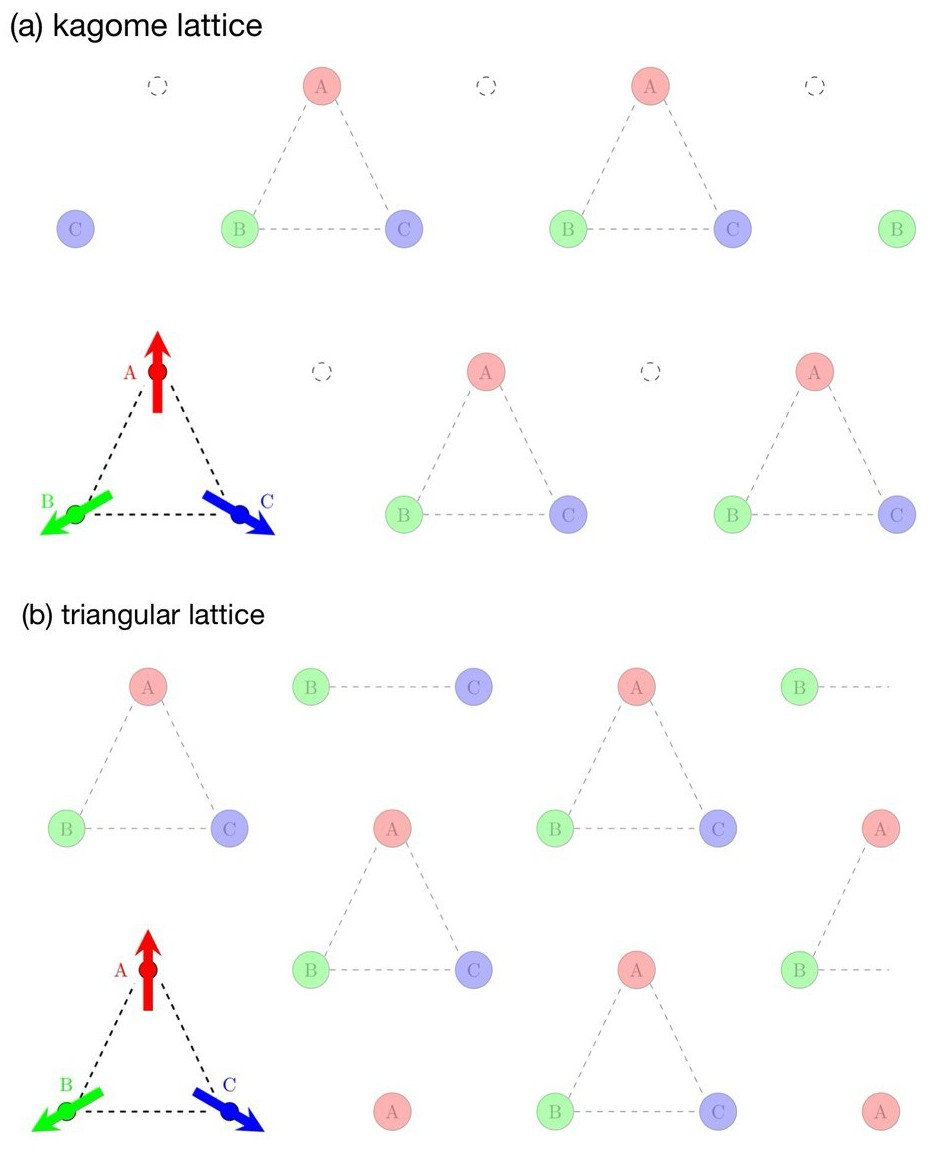
\includegraphics[width=1\linewidth]{img/kagome_triangular_11.jpg}
	\caption{Schematic image of (a) the kagome lattice and (b) the triangular lattice with non-collinear magnetic order. The three magnetic moments in the magnetic unit cell are shown in red (A), green (B) and blue (C). The net magnetic moment is zero. While the magnetic unit cell of both configurations is th same, the regular vacancy of the kagome lattice (dashed circle) distinguishes the two. In practice, the vacancy can be filled with a non-magnetic atom.}
	\label{fig:kagome_triangular}
\end{figure}


This paper is organized as follows: In Sec.~\ref{sec_modelling}, we
will introduce the model. In Sec.~\ref{sec_intrinsic}, we will discuss
intrinsic AMR (both for collinear MnN and for non-collinear AFMs),
followed by the discussion of extrinsic AMR in non-collinear AFMs
(Sec.~\ref{sec_extrinsic}). Details of ab initio calculations are
given in the appendix.

%{\color{red} What about ab initio}

%{\color{red} Potential weak point to only feature the real materials in intrinsic AMR}

\subsection{{\color{red} Symmetries, p-wave magnetism}}
{\color{red} A similar work was carried out by Tomas, Libor, Jairo named \textit{p-wave magnetism}~\cite{BirkHellenes:2023} and, at least, we have to find out how that affect the possible storyline of this paper. Some thoughts:

\begin{itemize}
	\item Significant overlap might be a problem: AMR ("spontaneous anisotropy of the resistivity") due to anisotropic Fermi surface, non-collinear materials, DFT example calculation, symmetry analysis
	\item On the other hand: Part of the (intrinsic AMR) results were shown in Sec. 4.2.3 of the review~\cite{Ritzinger:2023} and it can be argued that this paper is its "natural successor"
	\item The p-wave paper does NOT talk about: Rotation of the moments, extrinsic AMR; DFT with other material than ours
	\item Perhaps focus more on the results of the extrinsic AMR as its more unique and allows us to seperate from the overs. Any fancy explanation for the extrinsic result?
	\item I think it's still interesting to discuss why the non-compensated lattice works in the case of kagome, yet never in case of triangular
	\item P-wave paper mentions 73 material candidates (from magndata) identified to be such a p-wave magnet. The list is available in the supplementary material (not yet public??, at least I couldn't find it. It'd be interesting to compare to the materials we show here (MnN, Mn3Sn, CrSe)
	\item After all, the overlap doesn't need to be bad as we could also just say that we are consistent with the p-wave people and bring sth new to the table (other materials, extrinsic AMR, detail study of intrinsic and so on)
\end{itemize}
}

{\color{red} Check what's been done since 2212.03700
	(Fig. 16): there's perhaps something in 2309.01607 but otherwise, I can't find much searching for "anisotropic magnetoresistance (smejkal) jungwirth". PR 2025-04-03:
		
\begin{itemize}
	\item checked the keywords "AMR" or "resistivity" + "non-relativistic" in web of knowledge $\rightarrow$ nothing
	\item checked "p-wave magnetism" in web of knowledge and checked the paper that are citing 2309.01607. found TJ's latest paper (which he was also talking about in Sheffield): \textbf{2411.00717v2}
\end{itemize}	
	}



\section{Modelling}
\label{sec_modelling}

\subsection{Formalism}

We employ a simplistic tight-binding model which only consists of a hopping and an exchange term~\cite{Gonzalez-Hernandez:2024}:
\begin{equation}
H = -\sum_{i, j}\sum_\alpha t_{ij} {\hat{c}_i^{\alpha\dagger}} \hat{c}^\alpha_j + J \sum_{i} \sum_{\alpha, \beta} (\vec{\sigma} \cdot \hat{m}_i)_{\alpha \beta} {\hat{c}_i^{\alpha\dagger}} \hat{c}^\beta_i 
	\label{eq_sdmodel}
\end{equation} 
where $t_{ij}$ is the hopping parameter from site $i$ to $j$, $\alpha$ and $\beta$ are the spin indices, ${\hat{c}_i^{\alpha}}(^\dagger)$ is an annihilation (creation) operator at site $i$ with spin $\alpha$, $J$ is the Heisenberg exchange constant, $\vec{\sigma}$ the vector of the Pauli spin matrices and $\hat{m}_i$ the magnetization direction unit vector at site $i$.

The conductivity is then calculated using the Boltzmann equation~\cite{Vyborny:2009}. 

%\begin{equation}
\begin{multline}
	\sigma_{ij} = e^2 \sum_n  \int_ {1st BZ} \frac{d^3k}{(2\pi)^3} \delta(E_n(\vec{k}) - E_F) \frac{1}{\hbar \Gamma_{n, \vec{k}}} \times \\ v_{n,i}(\vec{k}) v_{n,j}(\vec{k})
	\label{eq_Boltzmann_1}
\end{multline}
%\end{equation}

where $e$ is the elementary charge, $E_n(\vec{k})$ is the k-dependent Eigen energy of the $n$th-band, $E_F$ is the Fermi energy, $\Gamma_{n, \vec{k}}$ is the scattering rate and $v_{n,i}$ is the $i$-th component of the Fermi velocity in the $n$-th band. The delta distribution evaluates the integral over the first Brillouin zone (1st BZ) at the Fermi surface. The Fermi velocity is calculated by:
%
\begin{equation}
v_{n, i} = \frac{1}{\hbar} \frac{\partial E_n(\vec{k})}{\partial k_i}
\end{equation}
%
The scattering rate is obtained by using Fermi's Golden Rule:
%
\begin{multline}
	\Gamma_{n, \vec{k}} = \frac{2 \pi}{\hbar} N_{scat} \sum_{n'}  \int_ {1st BZ} \frac{d^3k'}{(2\pi)^3} \delta(E_{n'}(\vec{k'}) - E_n(\vec{k})) \times \\ |M^{\vec{k}\vec{k'}}_{nn'} |^2 (1 - \cos \theta_{vv'})
	\label{eq_FermiGoldenRule_1}
\end{multline}

where $N_{scat}$ is the volume density of the scatterers, $M^{\vec{k}\vec{k'}}_{nn'}$ is the transition matrix element and $\cos \theta_{vv'} = \frac{\vec{v}_n (\vec{k})}{|\vec{v}_n (\vec{k})|}\frac{\vec{v}_n' (\vec{k'})}{|\vec{v}_n' (\vec{k'})|}$. The transition matrix element is calculated by:

\begin{equation}
	M^{\vec{k}\vec{k'}}_{nn'} = \langle \psi_{n, \vec{k}}|\hat{M}|\psi_{n', \vec{k'}} \rangle
	\label{eq_transmatrix}
\end{equation}

where $\psi_{n, \vec{k}}$ is the wave function for the Eigenenergy value $E_n(\vec{k})$~\cite{Vyborny:2009}. 

\subsection{Definition of AMR}

The anisotropy of resistance can be expressed as a percentage in the AMR ratio, thus $\Delta \rho / \rho \neq 0$~\cite{Ritzinger:2023} or by equivalently looking at the respective conductivities. There is two different ways, how this can be defined: Either we keep the magnetic order constant and then look at the conductivities at two different directions, e.g. $\sigma_{xx} / \sigma_{yy} \neq 1$ or we keep the direction of measurement constant, but rotate the magnetic order, e.g. $\sigma_{xx} (\vec{M_\perp})  / \sigma_{xx} (\vec{M_\parallel}) \neq 1$. Using the first configuration with the static magnetic order is usually more unhandy in experiment, but allows us to define the AMR as a spontaneous effect~\cite{Bakonyi:2022}. Utilizng this definition, we can understand that forms of non-relativistic AMR deviating from our definition exist, which can be illustrated at the example of the antiferromagnetic MnN, which consists of FM layers aligned antiparallel to each other~\cite{Dunz:2020}.

Another example of non-relativistic AMR can be found in antiferromagnetic EuTe$_2$. The material undergoes a metal-insulator transition (MIT), where the critical field and temperature is different in the \textit{ab}-plane than it is along the \textit{c}-axis. Measuring $\sigma_{xx}$ while rotating the magnetic field can then cause AMR of up to $40000\%$ due to the insuing MIT~\cite{Yang:2021}. Both of the latter examples, MnN and EuTe$_2$ are different mechanisms for non-relativistic AMR than in our approach utilizing non-collinear magnetic order.

Apart from AMR ratios, it is also possible to track angle-dependent MR which in its simplest form is shown in Eq.~\ref{eq_ncollAMR}. In FMs and collinear antiferromagnets, a single spin axis (SSA) exists, which is the magnetization and the N\'eel vector, respectively. It is assumed, that an applied magnetic field serves to rotate the SSA, which in turn creates the AMR signal. In non-collinear systems, no such SSA exist (that is, even if the applied magnetic field creates a small magnetization, the underlying magnetic order is still much more involved than in FMs). Interpretations of how AMR works are thus diverging: In Ref.~\onlinecite{Wu:2023} it is, for example, assumed that all spins are rotated at the same time by the magnetic field, ignoring possible tilts. Rotating all spins at the same time would not lead to any results in our case, since in absence of the SOC, the spin is not coupled to the lattice~\cite{Gonzalez-Hernandez:2024}. Also, AMR is due to the magnetic order and not due to orbital effects~\cite{Ritzinger:2023}, which is usually ensured by comparing measurements of longitudinal and transversal magnetoresistance (LMR and TMR, respectively)~\cite{Bakonyi:2022} or by assuming that saturation has been reached~\cite{Ritzinger:2021}. In non-collinear systems this can be more difficult as can be seen in the LMR and TMR measurements in Mn$_3$Sn in Fig. 5f of Ref.~\onlinecite{Chen:2021}, where the expected parallel course of LMR and TMR is not reached within the field range of up to roughly 10 T.

For the intrinsic AMR, we will rotate the magnetic moments individually, as a rotation of all moments simulatenously would not produce any effect due to missing SOC. This individual rotation can be justified by assuming that the magnetic field would be large enough to partially overcome the exchange interaction. For the extrinsic AMR, the moments are kept in their original position and we are either comparing $\sigma_{xx}$ with $\sigma_{yy}$, thus making use of the spontaneous effect definition; or we are only rotating the magnetic impurity while keeping all other moments at their position assuming that the impurity bound much less by exchange interaction than the regular moments. 

\subsection{An Expanded Phenomenological Model}

The angle-dependent form of AMR can be expressed phenomenologically in terms of power expansion of the magnetization direction~\cite{Doring:1938,Limmer:2008,DeRanieri:2008} and allows to describe even more complex crystalline AMR signals~\cite{Ritzinger:2021, Gonzalez-Betancourt:2024, NamHai:2012}. However, these models rely on the existence of a SSA as the magnetization or N\'eel vector. In non-collinear systems such SSA does not exist - even in case of weak ferromagnetism induced by an applied magnetic field, it would be likely an oversimplification to ignore the effects of the sublattices. "Local" treatment of effects is not new: For instance, basic AMR models in FMs rely on seperate contributions for spin up and spin down electrons (two-current models)~\cite{Ritzinger:2023}, or the Edelstein effect in non-collinear Mn$_3$Sn can be calculated for each sublattice~\cite{Gonzalez-Hernandez:2024}. Such local approach can be applied to AMR by considering the contributions of each magnetic sublattice (MSL) individually in the phenomenological model, which yields:

\begin{equation}
	\rho_{yy} = \rho_0 + \sum_{m = 1,2,3} \sum_{n = 2, 4, 6, ...} c_{m,n} \cos(n \alpha_m)
	\label{eq_sublattice_AMR}
\end{equation}
where $m$ is the index of the MSL, $n$ is the order of the spherical harmonic, $c_{m,n}$ is the index of the $n$-th harmonic of the $m$-th MSL, and $\alpha_m$ is the angle of the magnetization direction of the $m$-th magnetic moment (assuming an in-plane rotation). The coefficients $c_{m,n}$ can be obtained by fitting where for multiple MSLs measurements for different values of magnetic field $B$ are necessary. The position of the magnetic moments $\alpha_m$ can be obtained from SW models. While this is not going to be a main focus of this work, Eq.~\ref{eq_sublattice_AMR} together with an adequate SW model could help to distinguish the MCA from the AMR.



\section{Intrinsic AMR}
\label{sec_intrinsic}

As mentioned previously, intrinsic AMR means that the anisotropy of
the resistivity (or conductivity) $\sigma_{xx} / \sigma_{yy} \neq 1$
(or simply $\sigma_{xx} \neq \sigma_{yy}$) is of
scattering-independent origin. For now, we will exclude the option of scattering-dependent anisotropy by choosing the relaxation time approximation (RTA)\cite{Vyborny:2009_a} and replace Eq.~\ref{eq_FermiGoldenRule_1} by:
\begin{equation}
	\tau = \frac{1}{\hbar \Gamma_{n, \vec{k}}}
\end{equation}
where the relaxation time $\tau$ is constant and thus isotropic. This
means that the anisotropy can only enter through the Fermi velocity
contribution (or anisotropic plasma frequencies $\omega^p$). We can simplify Eq.~\ref{eq_Boltzmann_1} to:
%
\begin{equation}
	\sigma_{ii} \propto \int_ {FS} \sum_n   dk_F  v^2_{n,i}(\vec{k_F})
        \propto (\omega_{ii}^p)^2
	\label{eq_Boltzmann_2}
\end{equation}
%
where $\vec{k_F}$ is the wave vector at the Fermi surface (Fermi
vector).
% what about anisotropic Fermi surfaces !?!?  then there's no single k_F
We made use of the facts that we only consider the
longitudinal conductivity $\sigma_{ii}$ in two dimensional systems,
the delta distribution evaluates the integral over the first Brillouin
zone at the Fermi surface (FS), and the scattering rate is obtained by
RTA. $\sigma_{xx} \neq \sigma_{yy}$ if the integral of $\sum_n
v^2_{n,x}$ and $\sum_n v^2_{n,y}$ over the Fermi circle are not the
same. This is generally achieved by anisotropic Fermi surfaces,
whereas the FS must neither be spherical (which is perfect isotropic)
nor show the symmetry of the system, since the conductivity must
reflect the crystal symmetry due to Neumann's
principle~\cite{Ritzinger:2021} (e.g. a hexagonal FS in a hexagonal
material is insufficient). The results are summarized in the following
subsections, starting with the cubic collinear AFM MnN and
then proceeding to kagome lattice.

\subsection{Anisotropy due to magnetic order in collinear systems}

As discussed by Granville et al.~\cite{g} %PRB 72,205127 (or possibly earlier), 
MnN is a cubic
(rock-salt) crystal which, were it not for magnetic order, would have
$\sigma_{xx}=\sigma_{yy}=\sigma_{zz}$. The cation (manganese)
magnetic moments, however, prefer an A-type AFM order and in choosing
the direction of the ferromagnetic planes (e.g. $xy$-planes),
anisotropy arises (in that case, $\sigma_{zz}$ is different from
$\sigma_{xx}=\sigma_{yy}$). This effect in itself is non-relativistic in nature.
Calculations based on density functional theory (DFT as 
detailed in Appendix A, $a=b=c$), show that
$\hbar\omega^p_{xx}=5.87$~eV and $\hbar\omega^p_{zz}=5.23$~eV so that,
assuming isotropic scattering, $\sigma_{xx}/\sigma_{zz}-1\approx 26$~\%
according to~(\ref{eq_Boltzmann_2}).

Magnetic order leads to a distortion of lattice but this effect has only
minor influence on such transport anisotropy --- for example,
$a/c=0.4256/0.4189$~nm changes $\hbar\omega^p_{xx}$ to $5.88$~eV and
$\hbar\omega^p_{zz}$ to 5.10~eV.


\subsection{Kagome lattice}
\label{sec_I_Kagome}

\begin{figure}
	\centering
	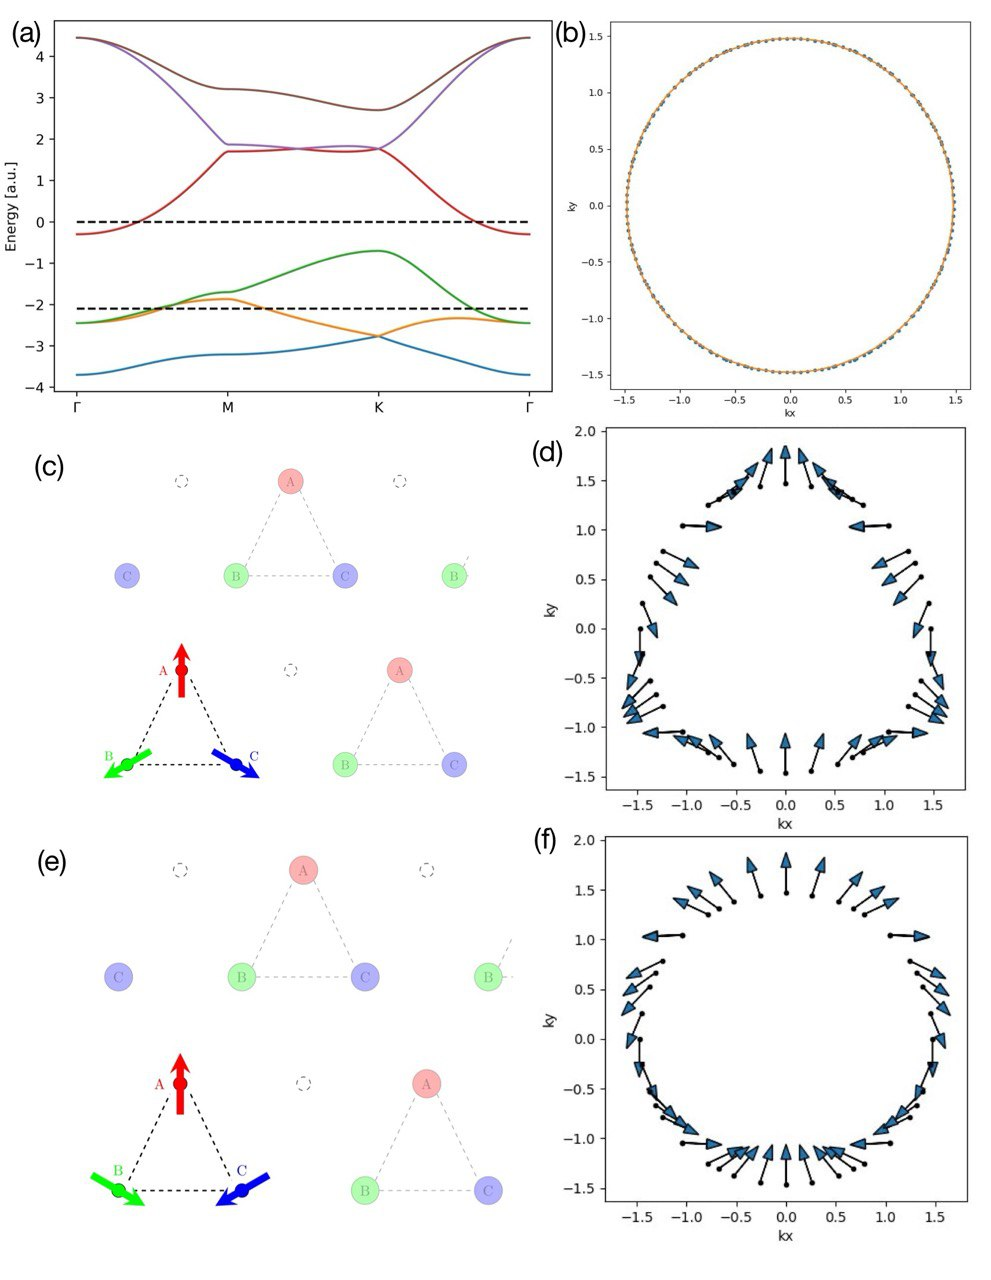
\includegraphics[width=1\linewidth]{img/overview_Kagome_phase1a}
	\caption{Results for two compensated magnetic configuration on the kagome lattice. (a) The band structure is spin-split. Permutation of magnetic moments does not change the bandstructure. (b) The Fermi surface at $E_F = 0$ (as indicated by the dashed line in (a)) is represented by the blue dots. The orange circle is shown for illustration. Since the FS and the circle overlap, this system has an isotropic FS and does not show intrinsic AMR. (c), (e) The magnetic unit cells of two compensated magnetic configurations and (d), (f) their respective k-space spin texture at the same Fermi level. While the band structure and Fermi surface is unaffected by permutation within the magnetic unit cell, the spin texture changes. The spin texture is entirely in the \textit{xy}-plane. The $\hat{z}$-component (not shown) of the spin texture is zero.}
	\label{fig:totalkagomephase1a}
\end{figure}


Turning to non-collinear systems, we first start by considering magnetic configurations, which are not changing the principle properties of the system, meaning that all moments will remain in the $xy$-plane (coplanar) and the moments cancel out (hence the system is perfectly compensated). Starting from the original configuration of moments as shown in Fig.~\ref{fig:kagome_triangular} (a), there are two possibilities: First, by permutations, which one is shown in Fig.~\ref{fig:totalkagomephase1a}, and second, by rotating all moments at the simultaneously. In both cases, regardless the permutation or angle of rotation, intrinsic AMR cannot be found and furthermore the results are equivalent (as well in band structure and Fermi surface) to the results shown in
Fig.~\ref{fig:totalkagomephase1a}. This is, as mentioned prior, because due to the lack of SOC, spin and lattice are decoupled~\cite{Gonzalez-Hernandez:2024}. Nevertheless, as shown in Fig.~\ref{fig:totalkagomephase1a} (d) and (f), the spintexture changes depending on the permutation. 

\begin{figure}
	\centering
	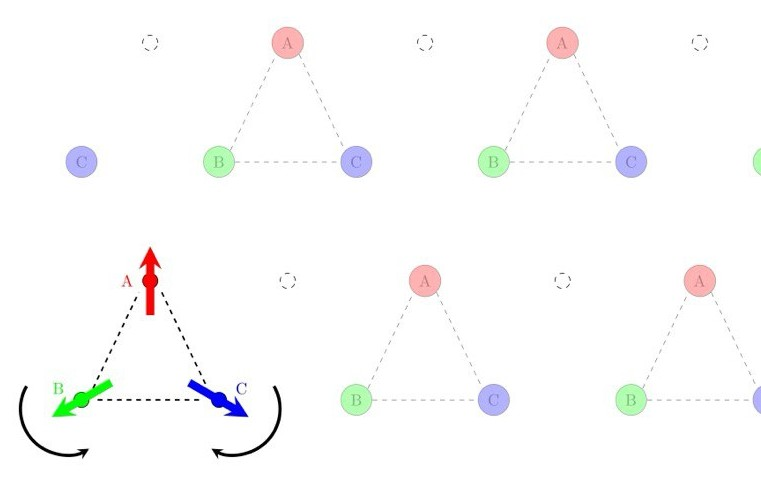
\includegraphics[width=0.9\linewidth]{img/kagome_rotation}
	\caption{Illustration of the rotation of the moments B (counterclockwise) and C (clockwise) by the same angle $\alpha$}
	\label{fig:kagomerotation}
\end{figure}


In the next step, we are individually rotating the magnetic moments
within the $xy$-plane as shown in Fig.~\ref{fig:kagomerotation}: While moment $A$ remains fix, moment $B$ is rotated counterclockwise and moment $C$ is rotated clockwise, illustrating the effect of a magnetic field in $-\hat{y}$-direction. Moments $B$ and $C$ are rotated by the same angle $\alpha$. Using this notion, we would like to draw the attention to a few special cases: $\alpha = 0^\circ (120^\circ)$ corresponds to the compensated states shown in Fig.~\ref{fig:totalkagomephase1a} (c) (Fig.~\ref{fig:totalkagomephase1a} (e)), $\alpha = 240^\circ$ corresponds to the ferromagnetic states with magnetization along $+\hat{y}$ and $\alpha = 60^\circ$ corresponds to a collinear ferrimagnetic state. For all $\alpha \neq 0^\circ, 120^\circ, 240^\circ$ a partially compensated in-plane magnetization, or weak ferromagnetism (WF), exists. We found an anisotropic FS as shown in Fig.~\ref{fig:asymmFS} and thus intrinsic AMR for all WF cases, which we attribute to the the broken rotation symmetry (the MSLs transform no longer one into another). Interestingly, all WF cases except the ferrimagnetic case are non-collinear. The anisotropic FS in case of the collinear ferrimagnetic case indicates that the {\color{red} non-collinear magnetic order is not needed to generate the effect, given that symmetry is low enough.} The magnetization in the WF cases is likely not sufficient to be a SSA, as mentioned before, but might play a role as a "symmetry breaking parameter". Similar results were observed in MnTe, where a besides the collinear antiferromagnetic ordering, a weak ferromagneticlike signal (WFL) was observed. The AHE in MnTe was not attributed due to the WFL, however the AHE is due to an imbalance of magnetic domains with Hall contributions that cancel out. This imbalance causes the WFL and thus the WFL serves as measure of this imbalance~\cite{Kluczyk:2024}, similar to our magnetization serving as measure of the symmetry breaking.

\begin{figure}
	\centering
	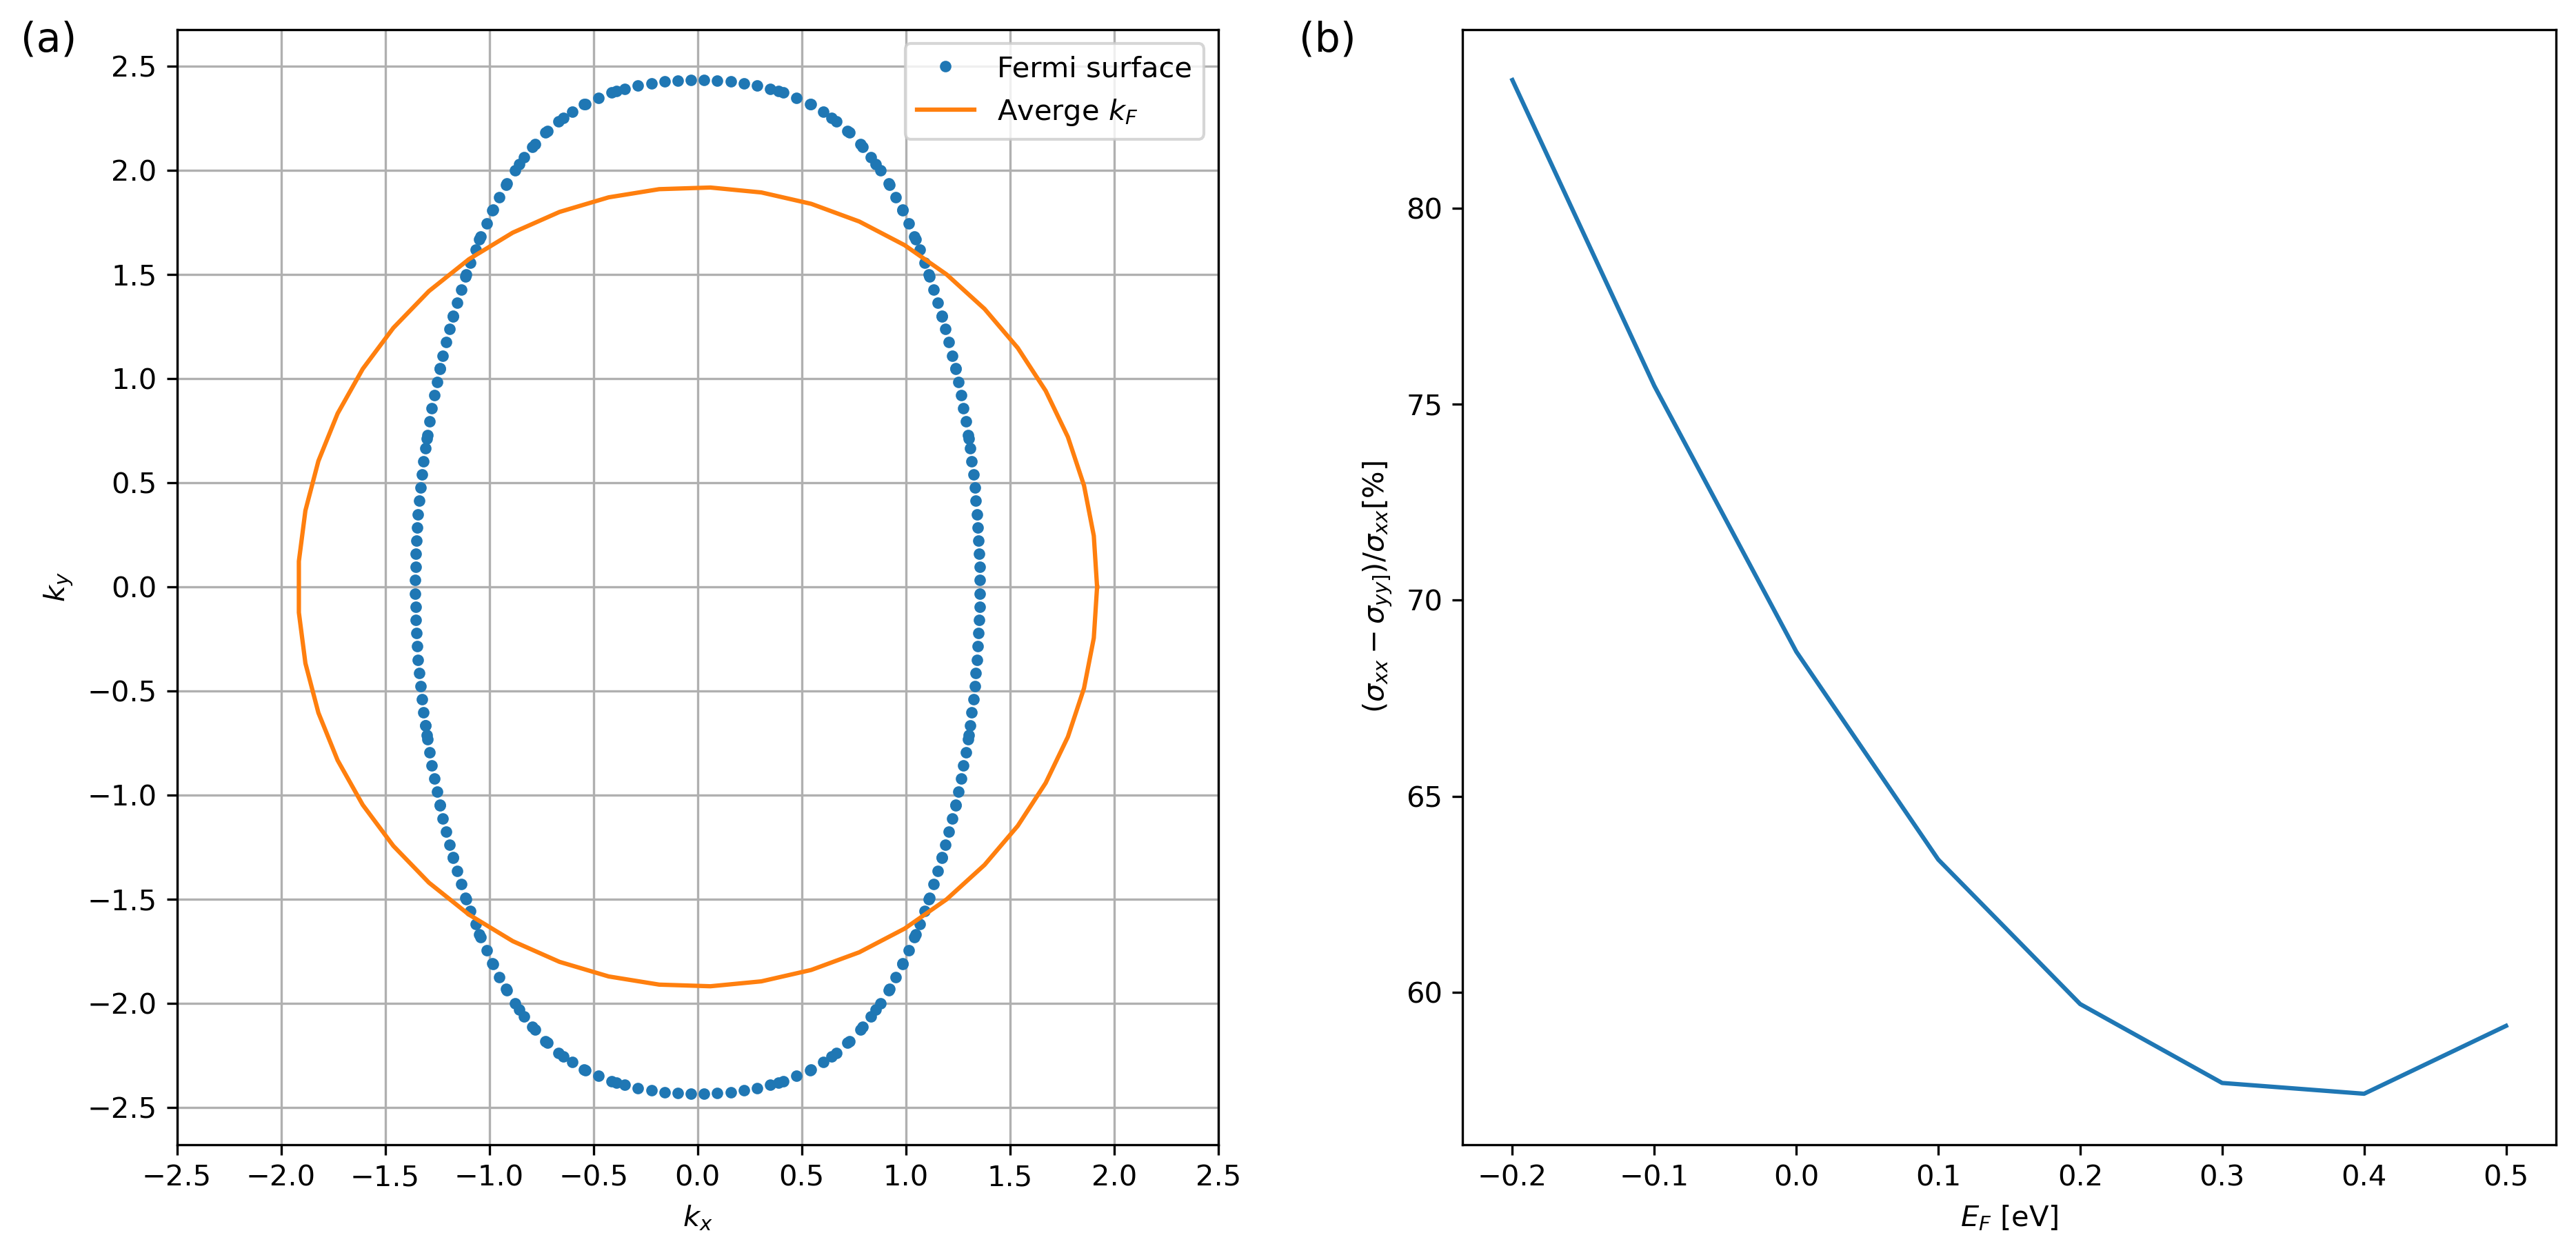
\includegraphics[width=\linewidth]{img/fig4_new}
	\caption{Anisotropy induced by magnetic order. The magnetic configuration corresponds to a rotation of the green and blue moments by by~$\alpha = 36^\circ$ as shown in Fig.~\ref{fig:kagomerotation} (or \ref{fig:fs-rotation} (a)). The small magnetization that ensues can serve as a measure of symmetry breaking. 		
	(a) Fermi surface (blue) at $E_F = 0.1$ showing a pronounced anisotropy between $\hat{x}$ and $\hat{y}$-directions. The orange circle is shown as reference.	
	(b) AMR vs. Fermi energy in the same system. Despite being a qualitative model, limited quantitative statements are possible. Energy scale directly comparable to Fig.~\ref{fig:totalkagomephase1a} (a)}
   \label{fig:asymmFS}
\end{figure}

We are now proposing an experiment to show this effect: Applying the magnetic field along a symmetry axis will tilt the magnetic moments, generate a weak ferromagnetic moment (magnetization) and result in AMR due to an anisotropic Fermi surface (see Fig.~\ref{fig:asymmFS} (a) and (c), ochre). Now, we are rotating the magnetic field by $120^\circ$, so that it points along another symmetry axis. The magnetic moments will tilt in another direction (see Fig.~\ref{fig:asymmFS} (b)), and result in a rotated FS, which does not overlap with the previous FS (see Fig.~\ref{fig:asymmFS} (c)), thus leading to another value of AMR. We can now rotate the conductivity measurement from $\sigma_{xx}$ and $\sigma_{yy}$ to $\sigma_{VV}$ and $\sigma_{WW}$, where here $\hat{V} = \hat{x} + 120^\circ$ ($\hat{W} = \hat{y} + 120^\circ$) and recover the original value of the AMR. 

\begin{figure}
	\centering
	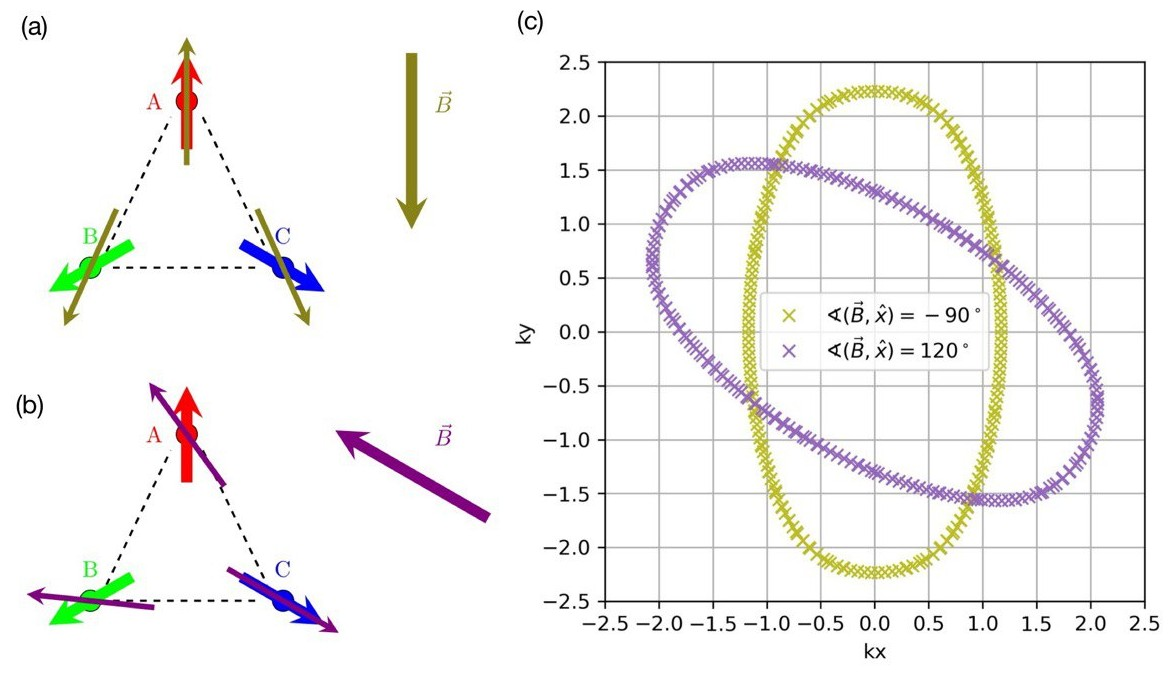
\includegraphics[width=1\linewidth]{img/FS-rotation}
	\caption{Rotation of the warped Fermi surface: 
	%	
	(a) The magnetic field (ochre) was applied in $-\hat{y}$-direction (or $\sphericalangle (\vec{B}, \hat{x}) = -90^\circ$) rotating the moments B and C towards the magnetic field, while leaving A in its original positions. The rotated moments are shown in ochre. (b) Simultaneously, the magnetic field (violet) was applied along $\sphericalangle (\vec{B}, \hat{x}) = 120^\circ$. The rotated moments are shown in violet. (c) The resulting Fermi surfaces (ochre and violet, respectively) are hence rotated by 60$^\circ$, and are not overlapping, resulting in a differing AMR.}
	\label{fig:fs-rotation}
\end{figure}


%{\color{red} Hold on: What IF the in-plane magnetization is actually the cause of the AMR? See AMR in FM: as in Eq.~\ref{eq_ncollAMR} where $\alpha$ is the angle of rotation of magnetization. What if here: the small emerging magnetization is indeed the order parameter and the ncoll order is replacing simply the SOC?}

\subsection{Triangular lattice}
\label{sec_I_triangular}

In case of the triangular lattice, the same operations were applied as for the kagome lattice. In both the compensated states and the non-compensated states show no anisotropic Fermi surface and hence, intrinsic AMR could not be found in this system. We attribute this to a higher symmetry the system shows {\color{red} which one? And what more?}

\subsection{CrSe and Mn$_3$Sn}
\label{sec_I_mat}

Now we are moving towards the real materials CrSe and Mn$_3$Sn. CrSe has a double layer triangular lattice, where the in-plane magnetic moments within each plane cancel out. The magnetic moments have an out-of-plane component, which gives every individual plane an out-of-plane moment, which is canceled out in the entire system since the out-of-plane component of the second plane is oriented antiparallely. The three-dimensionality of the components render CrSe non-coplanar. Secondly, we investigated Mn$_3$Sn, which has a double layer kagome lattice. The in-plane magnetic moments within each plane cancel out. There is no out-of-plane component of the magnetic moment, which makes it a coplanar, non-collinear magnetic.

Our prodecure is very similar to the procedure of the toy models: We first looked at the compensated cases, which, for both triangular CrSe and kagome Mn$_3$Sn did not yield any anisotropy. This is analogous to previous results. Then, we simulated an in-plane field along $+\hat{x}$-direction, leading to a tilt of magnetic moments and a weak non-zero in-plane magnetization. In case of CrSe, just like in the triangular toy model case, no anisotropy was generate, while for Mn$_3$Sn (see Fig.~\ref{fig:mn3sn_36deg_FS}) a non-zero AMR was found.

\begin{figure}
	\centering
	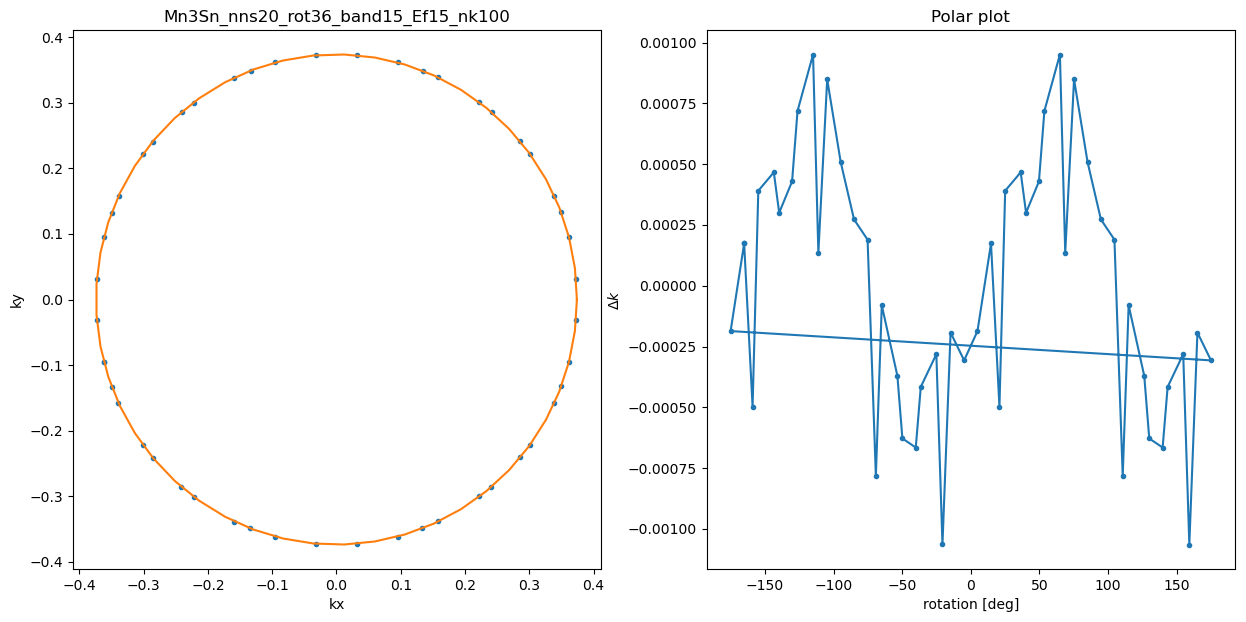
\includegraphics[width=\linewidth]{img/Mn3Sn_nns20_rot36_band15_Ef15_nk100}
	\caption{Fermi surface in the non-compensated case of Mn$_3$Sn at $E_F = 15$: (a) Fermi surface (blue) and for illustrative reasons a circle (orange). It seems as if they are overlapping and thus, an isotropic FS exists. (b) Deviation of the FS (blue dots in (a)) from the spherical symmetry (orange in (a)): A weak two-fold symmetry is recognizable, which is sufficent to reder the FS sufficiently anisotropic and create AMR {\color{red} (c) Magnetic configuration (missing) - Shall this plot be included?}}
	\label{fig:mn3sn_36deg_FS}
\end{figure}



\section{Extrinsic AMR}
\label{sec_extrinsic}

Now, we are going to move towards the extrinsic AMR. In this section we will revert to the full treatment of scattering via Eq.~\ref{eq_FermiGoldenRule_1}. We will assume magnetic impurities pointing in $\vec{i}$-direction described by the transition matrix matrix $\hat{M} = \hat{S}_i \otimes \hat{1}_{NxN}$, where $\hat{S}_i$ is the $i$-th Pauli spin matrix and $\hat{1}_{NxN}$ is the $N$-dimensional identity matrix. For simplicity reasons, we will restrict ourselves to impurities either pointing along $\hat{x}$, as illustrated in Fig.~\ref{fig:kagome21}, which shall be abbreviated as $\hat{x}$-impurities henceforth, and impurities along $\hat{y}$, denoted as $\hat{y}$-impurities.

\begin{figure}
	\centering
	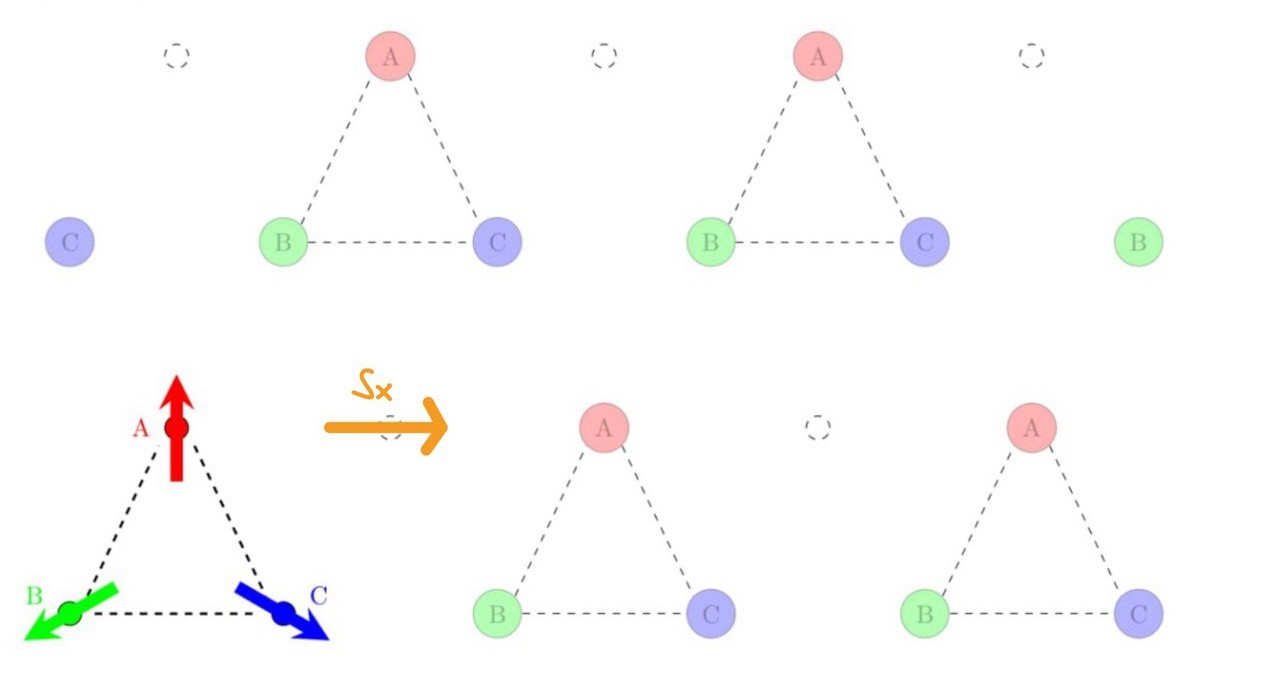
\includegraphics[width=0.8\linewidth]{img/Kagome_21}
	\caption{Illustration of a x-impurity in a kagome lattice}
	\label{fig:kagome21}
\end{figure}


Here, we are choosing three types of setups: A kagome lattice, a triangular lattice, and as reference a square lattice with a ferromagnetic order in $\hat{y}$-direction. We then calculate the conductivities $\sigma_{xx}$ and $\sigma_{yy}$ using the Eqs.~\ref{eq_Boltzmann_1}-\ref{eq_transmatrix}. The results are summarized in table~\ref{T_extrinsic}.

\begin{table}
	\begin{tabular}{llll}
	Lattice & Impurity $\hat{M}$ & AMR? & Spin texture \\
	\hline 
	\textbf{Kagome} & \textbf{X} & \textbf{Yes} & XY\\
	\textbf{Kagome} & \textbf{Y} & \textbf{Yes} & XY \\
	\textbf{Kagome (non-comp.)} & \textbf{X} & \textbf{Yes} & XY\\
	\textbf{Kagome (non-comp.)} & \textbf{Y} & \textbf{Yes} & XY \\
	\hline 
	Triangular & X & divergent & Z \\
	Triangular & Y & divergent & Z \\
	{\color{red} Triangular (non-comp.)} & {\color{red} X} & {\color{red} No} & {\color{red} ZY} \\
    Triangular (non-comp.) & Y & No & ZY \\
	\hline
	Square FM & X & divergent & Y\\
	Square FM & Y & No & Y
\end{tabular}
\caption{Results of the extrinsic AMR calculations for the various types of lattices and impurities as introduced in the text. "Yes" means that AMR was found, hence $\sigma_{xx} \neq \sigma_{yy}$ while for "No" an isotropic behavior was identified, where $\sigma_{xx} = \sigma_{yy}$. The value of the AMR ratio is not stated here, as our model is qualitative and quantitative values would not have any real meaning. Divergent means that both $\sigma_{xx}$ and $\sigma_{yy}$ are divergent or infinite and AMR cannot be defined, originating from a suppressed scattering rate $\Gamma \rightarrow 0$. "Spin texture" indicates the active components of the k-space spin texture at the Fermi surface. XY indicates that all the spins are within the XY plane and thus $\hat{s}_z = 0$ for all spins. The spin texture serves as a good intuition for whether a certain impurity would lead to suppressed scattering.}
\label{T_extrinsic}
\end{table}

In the kagome case, for both the $\hat{x}$- and the $\hat{y}$-impurity in both the compensated and non-compensated case, non-zero AMR can be found. In the triangular case, no AMR has been identified at all. In case of the square FM lattice, no AMR was found at all. In some cases the results in Tab.~\ref{T_extrinsic} are denoted by \textit{divergent}, which means that both $\sigma_{xx}$ and $\sigma_{yy}$ are divergent or infinite. This originates from a suppressed scattering due to that impurity $\Gamma \rightarrow 0$ and the fact that the inverse scattering rate is part of the Boltzmann equation Eq.~\ref{eq_Boltzmann_1}. Since our model is very simplistic, it is, however, not expected that in a real system the conductivity would diverge.

\begin{figure}
	\centering
	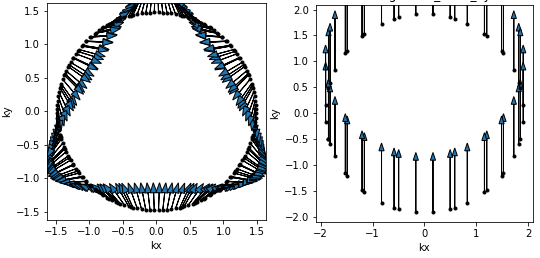
\includegraphics[width=1\linewidth]{img/Combined_Spintexture}
	\caption{The spintexture of the kagome (left) and square FM (right) lattice. In case of the square FM, all spins point in $+\hat{y}$-direction. The $\hat{z}$-component (not shown) is zero in both cases.}
	\label{fig:combinedspintexture}
\end{figure}

The momentum-space spintextures of the kagome lattice and the square FM are shown in Fig.~\ref{fig:combinedspintexture}. Spin textures can be an important tool as already shown in the context of the non-relativistic Edelstein effect~\cite{Gonzalez-Hernandez:2024}. {\color{red} Spin texture ref's: 14, 29, 34 for ncoll and 20-31 for coll in \cite{Gonzalez-Hernandez:2024}}. In our case, it can give us a hint about the possibility of AMR due to its similiarty: The $i$-th component of the spin texture is given by:

\begin{equation}
	S_i (\vec{k}) = \langle \psi_k | \hat{S_i} | \psi_k \rangle
\label{eq_spintexture}
\end{equation}

where $\psi_k$ is the wave function at $\vec{k}$. The scattering rate $\Gamma$ at the same $\vec{k}$ for a magnetic impurity in direction $i$ described by $\hat{S}_i$:

\begin{equation}	
{\Gamma_{\vec{k}}} \propto \int_{FS} dk' |\langle \psi_k |\hat{S_i}|\psi_k \rangle|^2
\label{eq_FermiGoldenRule_2}
\end{equation}

where in Eq.~\ref{eq_FermiGoldenRule_2} we ignored $\cos \theta_{vv'}$ and the prefactors, and the delta distribution was evaluated. The integration over $k_z$ does only contribute in a prefactor the system we are looking at is two dimensional. The resulting integral in Eq.~\ref{eq_FermiGoldenRule_2} is a one dimensional integral over the Fermi circle. As can be seen the scattering rate for a magnetic impurity in direction $i$ (Eq.~\ref{eq_FermiGoldenRule_2}) and the $i$-th component of the spin texture are looking very similar, except that the integral over the Fermi surface adds some level of complexity to it. Despite these small differences, it allows us to to explain a part of the results we find in Tab.~\ref{T_extrinsic}:

The spintexture of the square FM case (Fig.~\ref{fig:combinedspintexture} right panel) points exclusively in the $+\hat{y}$-direction, thus $s_x = 0$. In this case, introducing a $\hat{x}$-impurity will lead to a zero scattering rate or infinite conductivity, whereas a $\hat{y}$-impurity leads to a finite isotropic conductivity. The same is the case for the triangular lattice: The spin texture of the triangular lattice pointing along $+\hat{z}$ leading to a suppressed scattering for both $\hat{x}$- and $\hat{y}$-impurities.

%In case of the non-collinear triangular lattice, the moment space spin texture (not shown, similar to Fig.~\ref{fig:combinedspintexture} right panel) points to the $+\hat{z}$ direction. Yet still, a Z-impurity leads to an isotropic conductivity. The reason for this could be that while the impurity is applied in the $\hat{z}$-direction, the conductivity is measured in the xy-plane. There could be a non-zero AMR emerging if we look at the out-of-plane AMR $\sigma_{zz}/\sigma_{xx}$ instead. Since we are just looking at a two dimensional model, this would require changes to our model, however. 

Now, as a last part of this section, we can look at the crystalline AMR, which refers to the anisotropy of conductivity created by the crystalline symmetry. In our case, this can be defined as {\color{red} (redo the calculations to doublecheck)}:

\begin{equation}
	AMR^{cry}_{VW} = \frac{\sigma_{WW} (\hat{M} = \hat{W})}{\sigma_{VV} (\hat{M} = \hat{V})}
\end{equation}
 
where $V$ and $W$ are two arbitrary directions (e.g. $\hat{x}$ and $\hat{y}$). The crystalline AMR is thus defind as the quotient as the longitudinal conductivity in $V$ direction for a magnetic impurity in the same direction with the longitudinal conductivity along $W$ for a magnetic impurity in the same direction. In both numerator and denominator are thus longitudinal conductivities with parallel aligned impurity. The resulting anisotropy $AMR^{cry}_{VW} \neq 1$ would thus arise only from the influence of the crystal directions. Calculating the respective quantities for the kagome lattice, we indeed find non-zero crystalline AMR.

\section{Conclusions}

Summary and conclusion

\begin{itemize}
	\item more materials could be investigated, e.g. $\delta$-FeMn
	or RbFe(MoO$_4$)$_2$
	\item All in all, it has to be kept in mind that the model we are using is highly simplistic in its nature. First, the model only contains a hopping and a Heisenberg exchange term. More realistic and complex contributions to systems, such as different atomic orbitals, the crystal field, or the contributions of phonons and magnons, are ignored, as well as any kind of many-body interactions and correlations. For the model systems (thus not in the materials), we also only look into next-neighbor hopping. In the exchange, more complicated (often mid-range) pairings of moments are ignored as well as higher-order contributions such as Dzyaloshinsky-Moriya interaction, which can play a role in such non-collinear systems. It has to be reminded that the spin moments are not just dipole arrows pointing in an direction, but they are spin densities, which contain also higher multipoles
	\item look at triangular and kagome with e.g. 9 moments in magnetic unit cell. 
	\item propose some experimental method: AMR is traditionally known to be dependent on SOC - it was considered crucial to maximize the SOC to maximize AMR~\cite{Ritzinger:2023}. While SOC cannot be "turned off", we can talk about scaling effects: E.g. finding somewhere (in the classics) how AMR scales with SOC. Then looking at an analogous effect, e.g. AHE and look at Mn$_3$X (X = Ge~\cite{Kiyohara:2016}, Sn~\cite{Nakatsuji:2015}, Ir~\cite{Iwaki:2020}), where the atomic number of these 3 is very different $\rightarrow$ doesnt scale with SOC. Need to find something similar for AMR. Also, ab initio can give rise (compare to \cite{Gonzalez-Hernandez:2024} - also, there are spin currents in Mn3Sn and -Ge \cite{Zelezny:2017}. The discussion is really good there, take some inspiration and refer to it)
	
	\item stronger take home message?
	\item p-wave magnetism and our paper ... 
\end{itemize}


\section*{Acknowledgments}

Our work benefited from discussions with folks interested in AMR...
we express our gratitude to them as well as to funding sources from GA\v{C}R (under contract 22-21974S).
 
\begin{appendix}

\section{Ab initio calculations}

$\hbar\omega^p_{xx}=5.87$~eV and $\hbar\omega^p_{zz}=5.23$ for MnN
were obtained using GGA with SO under assumption of 'perfectly cubic
lattice constants'; when SO is switched off, we get similar anisotropy...

\section{Commentary about the Tight-Binding Model}

From Fig.~\ref{fig:asymmFS} (b), we can see that within our model, limited quantitative statements are possible, at least as long we are keeping within the same lattice and magnetic configurations and keep to a sufficiently small regime. Comparing AMR values quantitatively at vastly different Fermi levels (and thus bands), or the same Fermi levels for different magnetic configuration, or even between different lattices, leads to jumps in the numerical value and does thus not provide ground for a useful analysis. On the contrary, a qualtitative statement is always possible: Given a certain lattice and magnetic configuration, in an isotropic case $\sigma_{xx} / \sigma_{yy} = 1$ for all Fermi energies in all bands, and in an anisotropic case, $\sigma_{xx} / \sigma_{yy} \neq 1$ for all Fermi energies in all bands (although the precise value of $\sigma_{xx} / \sigma_{yy}$ in the anisotropic case is very sensitive to small parameter changes). With changing Fermi level $E_F$, the form of the FS might change as illustrated in Fig.~\ref{fig:kagomenns1phase1adphi0band3ef1}.


\begin{figure}
	\centering
	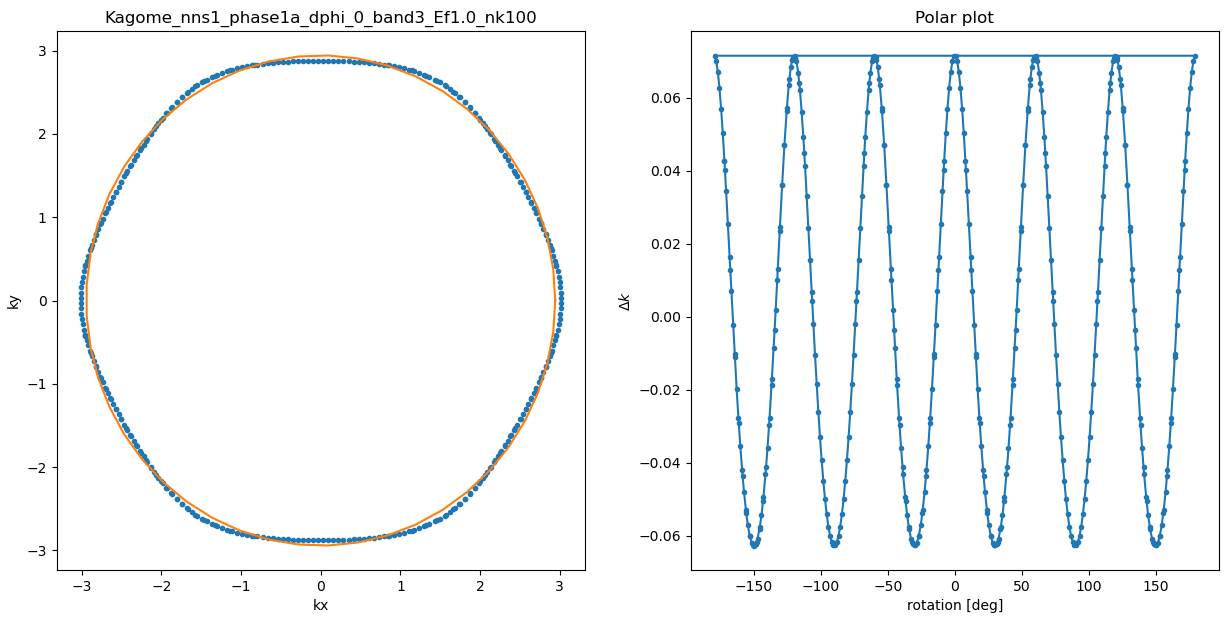
\includegraphics[width=\linewidth]{img/Kagome_nns1_phase1a_dphi_0_band3_Ef1.0_nk100}
	\caption{Fermi surface for the compensated configuration of the Kagome lattice (see Fig.~\ref{fig:totalkagomephase1a} (b)) for a different Fermi level ($E_F = 1$). The FS becomes more hexagonal, which is still isotropic with regards to the conductivity tensor.}
	\label{fig:kagomenns1phase1adphi0band3ef1}
\end{figure}



While in both toy models (kagome lattice, see Sec.~\ref{sec_I_Kagome}, and triangular lattice, see Sec.~\ref{sec_I_triangular}), we only took next neighbor hopping into account, in the material systems (CrSe and Mn$_3$Sn, see Sec.~\ref{sec_I_mat}), this did not lead to any realistic results. For CrSe we took the ten next neighbors into account, for Mn$_3$Sn 20. We chose this number by calculating the Fermi surface and AMR for the material systems using fully ferromagnetic moments as input. Since there is no SOC, the results should be isotropic, any anisotropy can be considered an artifact. We started by next neighbor hopping and increased the number of neighbors until isotropy in the FM state was reached.

\section{Further magnetic configuration in the kagome lattice {\color{red} - keep, or kick out?} }

\begin{figure}
	\centering
	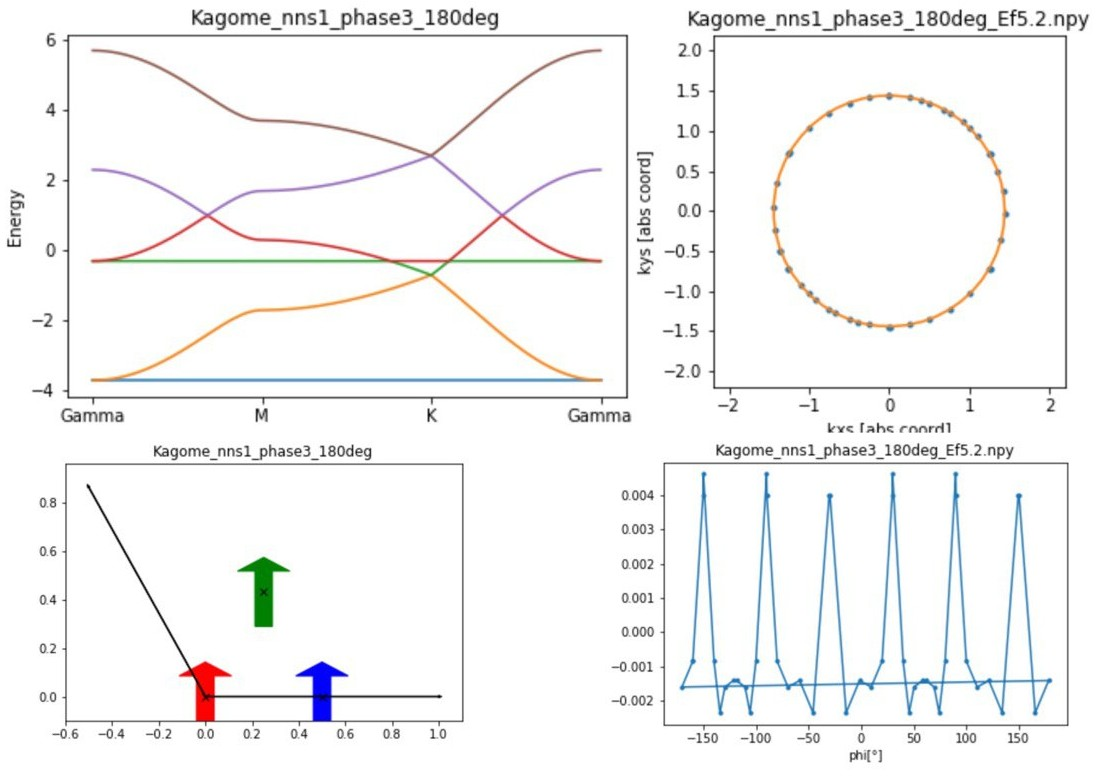
\includegraphics[width=0.9\linewidth]{img_total/total_Kagome_phase3_180}
	\caption{Results for the kagome lattice, where all moments point towards $+\hat{y}$ (FM state) (left lower panel). Left upper panel: The Bandstructure is still spin-split with two bands being flat (k-independent) on the shown k-range, which can be attibuted to the simplicity of the model. Right upper panel: The Fermi surface {\color{red} (Ef, band?)} is represented by the blue dots with the orange circle shown for illustration. The FS is isotropic. Right lower panel: Difference of the FS points the circle. The FS shows a small six-fold modulation on top of an almost perfect spherical symmetry. The system does not show intrinsic AMR. {\color{red} change color code of unit cell arrays: exchange red and green}}
	\label{fig:totalkagomephase3180}
\end{figure}

\begin{figure}
	\centering
	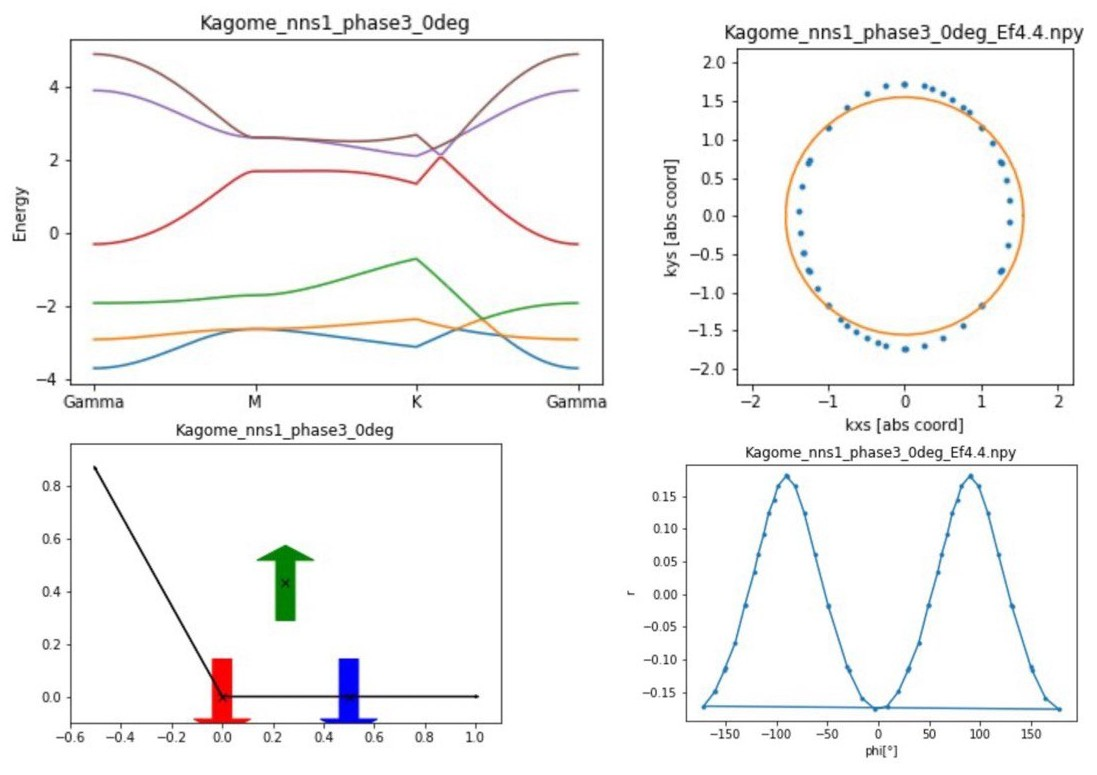
\includegraphics[width=0.9\linewidth]{img_total/total_Kagome_phase3_0}
	\caption{Collinear ferrimagnetic position. Elipsoid FS. AMR exists{\color{red} change color code of unit cell arrays: exchange red and green}}
	\label{fig:totalkagomephase30}
\end{figure}

\begin{figure}
	\centering
	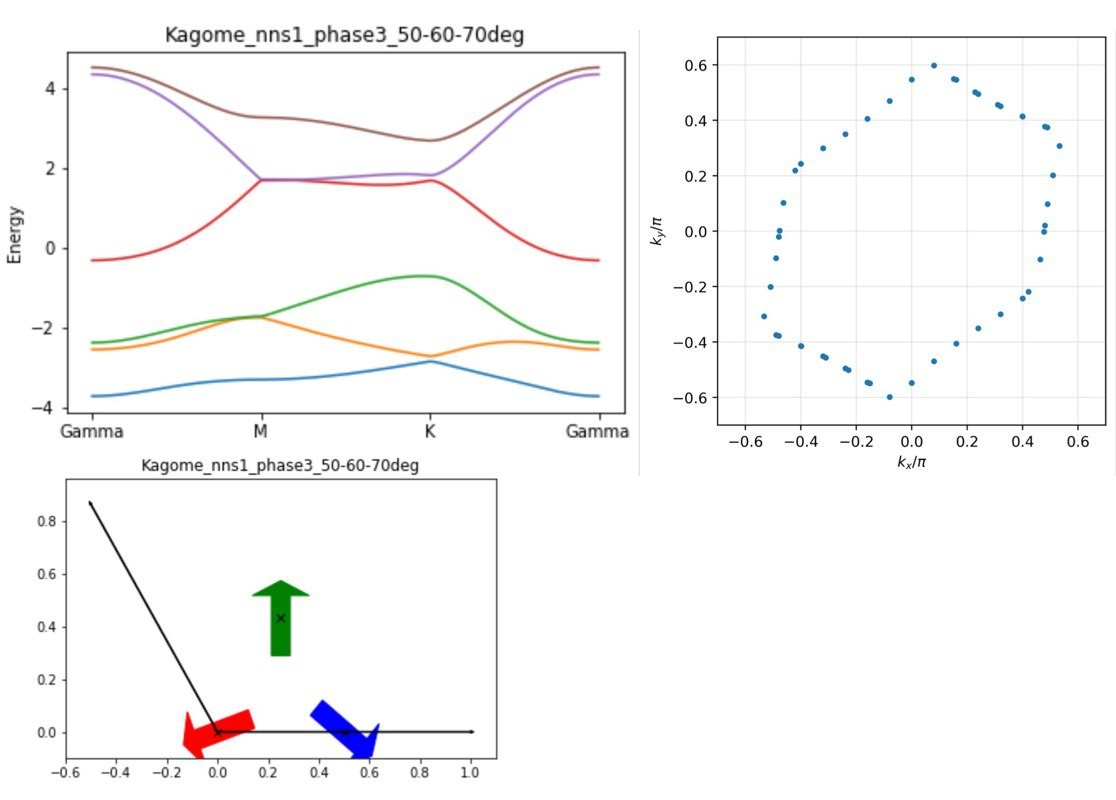
\includegraphics[width=0.9\linewidth]{img_total/total_Kagome_phase3_50-60-70}
	\caption{Red and blue moment manipulated leading to some non-compensated state. Warped hexagon is sufficiently anisotropic{\color{red} change color code of unit cell arrays: exchange red and green}}
	\label{fig:totalkagomephase350-60-70}
\end{figure}

\begin{figure}
	\centering
	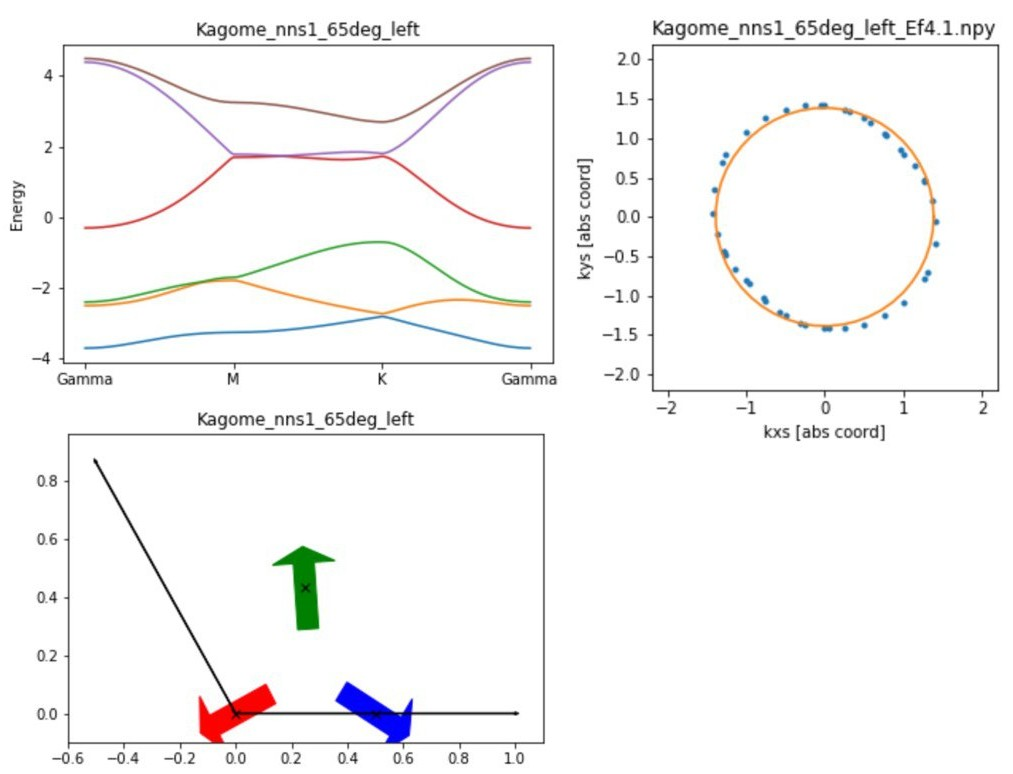
\includegraphics[width=0.9\linewidth]{img_total/total_Kagome_phase3_65L}
	\caption{Simulating magnetic field to the left (-x). Yes{\color{red} change color code of unit cell arrays: exchange red and green} }
	\label{fig:totalkagomephase365l}
\end{figure}



\end{appendix}

\def\urlprefix{}
\def\url#1{}\bibliography{lit}
%% %\bibliography{dms-assorted}% 


\begin{thebibliography}{99}

% cut after 20 authors


\bibitem{Thomson:1857} W. Thomson, Proc. R. Soc. Lond. 8, 546.(1857) %(doi:10.1098/rspl.1856.0144)

\bibitem{Ritzinger:2023} Philipp Ritzinger, Karel V\'yborn\'y, R. Soc. Open Sci., 10, 230564 (2023). %DOI: 10.1098/rsos.230564

\bibitem{Alagoz:2015} H. S. Alagoz, J. Desomberg, M. Taheri, F. S. Razavi, K. H. Chow, and J. Jung, Appl. Phys. Lett. 106, 082407 (2015)

\bibitem{McGuire:1975} T. McGuire, T. Potter. IEEE Trans. Magn. 11, 18 (1975) % (doi:10.1109/TMAG.1975.1058782)

\bibitem{Kriegner:2017} D. Kriegner, H. Reichlova, J. Grenzer, W. Schmidt, E. Ressouche, J. Godinho, T. Wagner, S. Y. Martin, A. B. Shick, V. V. Volobuev, G. Springholz, V. Hol\'{y}, J. Wunderlich, T. Jungwirth, and K. V\'{y}born\'{y}, Phys. Rev. B 96, 214418 (2017). %DOI: 10.1103/PhysRevB.96.214418

\bibitem{Gonzalez-Betancourt:2024} R. D. Gonzalez Betancourt, J. Zub\'a\v{c}, K. Geishendorf, P. Ritzinger, B. R\r{u}\v{z}i\v{c}kov\'a, T. Kotte, J. \v{Z}elezn\'y, K. Olejn\'ik, G. Springholz, B. B\"uchner, A. Thomas, K. V\'yborn\'y, T. Jungwirth, H. Reichlov\'a, and D. Kriegner, npj Spintronics, 2, 45 (2024). %DOI: 10.1038/s44306-024-00046-z


\bibitem{Volny:2020} J. Voln\'y, D. Wagenknecht, J. \v{Z}elezn\'y, P. Harcuba, E. Duverger–Nedellec, R. H. Colman, J. Kudrnovsk\'y, I. Turek, K. Uhl\'i\v{r}rov\'a, K. V\'yborn\'y, Phys. Rev. Mat. 4, 064403 (2020).% DOI: 10.1103/PhysRevMaterials.4.064403

\bibitem{Zubac:2021} J. Zub\'a\v{c}, Z. Ka\v{s}par, F. Krizek, F\"orster, R. P. Campion, V. Nov\'ak, T. Jungwirth, K. Olejn\'ik, Phys. Rev. B 104, 184424 (2021). %DOI: 10.1103/PhysRevB.104.184424

\bibitem{Wadley:2016} P. Wadley, B. Howells, J. \v{Z}elezn\'y, C. Andrews, V. Hills, R. P. Campion, V. Nov\'ak, K. Olejn\'ik, F. Maccherozzi, S. S. Dhesi, S. Y. Martin, T. Wagner, J. Wunderlich, F. Freimuth, Y. Mokrousov, J. Kune\v{s}, J. S. Chauhan, M. J. Grzybowski, A. W. Rushforth, K. W. Edmonds, B. L. Gallagher, T. Jungwirth, Science 351, 6273 (2016). %DOI: 10.1126/science.aab1031

\bibitem{Kabara:2017} K. Kabara, M. Tsunoda, S. Kokado, AIP Adv. 7, 056416 (2017). %DOI:10.1063/1.4974065

\bibitem{Doring:1938} W. D\"oring, Ann. Phys. 424, 259-276
(1938). %DOI: 10.1002/andp.19384240306

\bibitem{Vyborny:2009_a} K. V\'yborn\'y, A. A. Kovalev, J. Sinova, T. Jungwirth, Phys. Rev. B 79, 045427 (2009). % DOI: 10.1103/PhysRevB.79.045427
  
\bibitem{Ritzinger:2021} P. Ritzinger, H. Reichlov\'a, D. Kriegner, A. Markou, R. Schlitz, M. Lammel, D. Scheffler, G. H. Park, A. Thomas, P. St\v{r}eda, C. Felser, S. T. B. Goennenwein, and Karel V\'yborn\'y, Phys. Rev. B, 104, 094406 (2021)

\bibitem{Sato:2019} T. Sato, S. Kokado, M. Tsujikawa, T. Ogawa, S. Kosaka, M. Shirai, and M. Tsunoda, Appl. Phys. Express 12, 103005 (2019)

\bibitem{Limmer:2008} W. Limmer, J. Daeubler, L. Dreher, M. Glunk, W. Schoch, S. Schwaiger, R. Sauer, Phys. Rev. B 77, 205210 (2008). %DOI: 10.1103/PhysRevB.77.205210

\bibitem{DeRanieri:2008} E. De Ranieri, A. W. Rushforth, K. V\'yborn\'y, U. Rana, E. Ahmad, R. P. Campion, C, T, Foxon, B. L. Gallagher, A. C. Irvine, J. Wunderlich, New J. Phys. 10, 065003 (2008).% DOI: 10.1088/1367-2630/10/6/065003

\bibitem{NamHai:2012} P. Nam Hai, D. Sasaki, L. Duc Anh, M. Tanaka, Appl. Phys. Lett. 100, 262409 (2012). DOI:10.1063/1.4730955

\bibitem{Limmer:2006} W. Limmer M. Glunk, J. Daeubler, T. Hummel, W. Schoch, R. Sauer, C. Bihler, H. Huebl, M. S. Brandt, S. T. B. Goennenwein, Phys. Rev. B 74, 205205 (2006).% DOI: 10.1103/PhysRevB.74.205205

\bibitem{Dong:2023} M. Q. Dong, Z.-X. Guo , X. R. Wang, Phys. Rev. B 108, L020401 (2023). % DOI: 10.1103/PhysRevB.108.L020401

\bibitem{Nadvordnik:2021} L. N\'{a}dvorn\'{i}k, M. Borchert, L. Brandt, R. Schlitz, K. A. de Mare, K. V\'{y}born\'{y}, I. Mertig, G. Jakob, M. {Kl\"{a}ui}, S. T.B. Goennenwein, M. Wolf, G. Woltersdorf, T. Kampfrath, Phys. Rev. X 11, 021030 (2021). %DOI: 10.1103/PhysRevX.11.021030

\bibitem{Park:2021} J.‑H. Park, H.‑W. Ko, J.‑M. Kim, J. Park, S.‑Y. Park, Y. Jo, B.‑G. Park, S. K. Kim, K.‑J. Lee, K.‑J. Kim, Sci. Rep. 11, 20884 (2021).% DOI: 10.1038/s41598-021-00374-8

\bibitem{Bonbien:2022} Bonbien \textit{et al.} J. Phys. D: Appl. Phys. 55, 103002 (2022)

\bibitem{Gonzalez-Hernandez:2024} R. Gonz\'alez-Hern\'andez, P. Ritzinger, K. V\'yborn\'y, J. \v{Z}elezn\'y, and A. Manchon, Nat. Commun., 15, 7663 (2024).% DOI: 10.1038/s41467-024-51565-6

\bibitem{g} % the proper label should probably be Granville:2005_a or smth ~
S. Granville et al., Phys. Rev. B 72, 205127 (2005).

\bibitem{Vyborny:2009} K. V\'{y}born\'{y}, J. Ku\v{c}era, J. Sinova, A. W. Rushforth, B. L. Gallagher, T. Jungwirth, Phys. Rev. B 80, 165204 (2009)%. DOI: 10.1103/PhysRevB.80.165204

\bibitem{Corliss:1961} L. M. Corliss, N. Elliot, J. M. Hastings, R. L. Sass, \textit{Phys. Rev.} 122, 1402-1406 (1961). %DOI: 10.1103/PhysRev.122.1402

\bibitem{Polesya:2010} S. Polesya, S. Mankovsky, D. Benea, H. Ebert, W. Bensch, \textit{J. Phys.: Condens. Matter} 22, 156002 (6pp) (2010). %DOI: 10.1088/0953-8984/22/15/156002

\bibitem{Tajima:2024} Y. Tajima, J. Shiogai, K. Ueda, K. Kudo, J. Matsuno, \textit{APL Mater.} 12, 041112 (2024). %DOI: 10.1063/5.0201786

\bibitem{Yang:2020} C.-Y. Yang, L. Pan, A. J. Grutter, H. Wang, X. Che, Q. L. He, Y. Wu, D. A. Gilbert, P. Shafer, E. Arenholz, H. Wu, G. Yin, P. Deng, J. A. Borchers, W. Ratcliff II, K. L. Wang, \textit{Sci. Adv.} 6, eaaz8463 (2020). %DOI: 10.1126/sciadv.aaz8463

\bibitem{Yan:2017} J. Yan, X. Luo, F. C. Chen, Q. L. Pei, G. T. Lin, Y. Y. Han, L. Hu, P. Tong, W. H. Song, X. B. Zhu, Y. P. Sun, \textit{Appl. Phys. Lett.} 111, 022401 (2017). %DOI: 10.1063/1.4985224

\bibitem{Chen:2021} T. Chen, T. Tomita, S. Minami, M. Fu, T. Koretsune, M. Kitatani, I. Muhammad, D. Nishio-Hamane, R. Ishii, F. Ishii, R. Arita, S. Nakatsuji, \textit{Nat. Commun.} 12, 572 (2021). %DOI: 10.1038/s41467-020-20838-1

\bibitem{Manna:2018} K. Manna, Y. Sun, L. Muechler, J. K\"uebler, C. Felser, "Heusler, Weyl and Berry", \textit{Nat. Rev. Mater.} 3, 244-256 (2018). %DOI: 10.1038/s41578-018-0036-5

\bibitem{Nakatsuji:2015} S. Nakatsuji, N. Kiyohara, T. Higo, \textit{Nature} 527, 212–215 (2015). %DOI: 10.1038/nature15723

\bibitem{Sharma:2023} V. Sharma, R. Nepal, R. C. Budhani, \textit{Phys. Rev. B} 108, 144435 (2023). %DOI: 10.1103/PhysRevB.108.144435 

\bibitem{Cable:1993} J. W. Cable, N. Wakabayasi, P. Radhakrishna, \textit{Phys. Rev. B} 48, 6159 (1993). %DOI: 10.1103/PhysRevB.48.6159

\bibitem{Zhou:2020} X. F. Zhou, X. Z. Chen, Y. F. You, L. Y. Liao, H. Bai, R. Q. Zhang, Y. J. Zhou, H. Q. Wu, C. Song, F. Pan, \textit{Phys. Rev. Appl.} 14, 054037 (2020). %DOI: 10.1103/PhysRevApplied.14.054037

\bibitem{Ikhlas:2017} M. Ikhlas, T. Tomita, T. Koretsune, M.-T. Suzuki, D. Nishio-Hamane, R. Arita, Y. Otani, S. Nakatsuji, \textit{Nat. Phys.} 13, 1085. %DOI: 10.1038/NPHYS4181

\bibitem{Park:2018} P. Park, J. Oh, K. Uhl\'i\v{r}ov\'a, J. Jackson, A. De\'ak, L. Szunyogh, K. H. Lee, H. Cho, H.-L. Kim, H. C. Walker, D. Adroja, V. Sechovsk\'y, J.-G. Park, \textit{npj Quantum Materials} 3:63 (2018). %DOI: 10.1038/s41535-018-0137-9.

\bibitem{Zelezny:2017} J. \v{Z}elezn\'y, Y. Zhang, C. Felser, B. Yan, \textit{Phys. Rev. Lett.} 119, 187204 (2017). %DOI: 10.1103/PhysRevLett.119.187204

\bibitem{Wu:2023} M. Wu, K. Kondou, T. Chen, S. Nakatsuji, Y. Otani, \textit{AIP Adv.} 13, 045102 (2023). %DOI: 10.1063/5.0138208

\bibitem{Reichlova:2019} H. Reichlova, T. Janda, J. Godinho, A. Markou, D. Kriegner, R. Schlitz, J. Zelezny, Z. Soban, M. Bejarano, H. Schultheiss, P. Nemec, T. Jungwirth, C. Felser, J. Wunderlich,  S.T.B. Goennenwein, \textit{Nat. Commun.} 10:5459 (2019). %DOI: 10.1038/s41467-019-13391-z

\bibitem{Zhang:2017} Y. Zhang, Y. Sun, H. Yang, J. \v{Z}elezn\'y, S. P. P. Parkin, C. Felser, B. Yan, \textit{Phys. Rev. B} 95, 075128 (2017). %DOI: 10.1103/PhysRevB.95.075128

\bibitem{Nagaosa:2010} N. Nagaosa, J. Sinova, S. Onoda, A. H. MacDonald, N. P. Ong, \textit{Rev. Mod. Phys.} 82, 1539 (2010). %DOI: 10.1103/RevModPhys.82.1539
    
\bibitem{Bakonyi:2022} I. Bakonyi, F. D. Czeschka, L. F. Kiss, V. A. Isnaini, A. T. Krupp, K. Palot\'as, S. Zsurzsa, L. P\'eter, arXiv:2203.11568 [cond-mat.mtrl-sci] (2022). %DOI: 10.48550/arXiv.2203.11568.

\bibitem{Kato:2008} T. Kato, Y. Ishikawa, H. Itoh, J.-i. Inoue, Phys. Rev. B 77, 233404 (2008). %DOI: 10.1103/Phys-RevB.77.233404

\bibitem{Velev:2005} J. Velev, R. F. Sabirianov, S. S. Jaswal, E. Y. Tsymbal, Phys. Rev. Lett. 94, 127203 (2005). %DOI: 10.1103/PhysRevLett.94.127203

\bibitem{Zeng:2020} F. L. Zeng, Z. Y. Ren, Y. Li, J. Y. Zeng, M. W. Jia, J. Miao, A. Hoffmann, W.Zhang, Y. Z. Wu, Z. Yuan, Phys.Rev. Lett. 125, 097201 (2020). %DOI: 10.1103/PhysRevLett.125.097201

\bibitem{Kato:2007} T. Kato, Y. Ishikawa, H. Itoh, J. Inoue, phys. stat. sol. (b) vol. 244, 12, 4403 - 4406 (2007). %DOI:10.1002/pssb.200777260

\bibitem{Iwaki:2020} H. Iwaki, M. Kimata, T. Ikebuchi, Y. Kobayashi, K. Oda, Y. Shiota, T. Ono, T. Moriyama,  Appl. Phys. Lett. 116, 022408 (2020). %doi: 10.1063/1.5128241

\bibitem{Kiyohara:2016} N. Kiyohara, T. Tomita, S. Nakatsuji, Phys. Rev. Appl. 5, 064009 (2016). DOI: 10.1103/PhysRevApplied.5.064009

\bibitem{Dunz:2020} Dunz et al. MnN, DOI: 10.1103/PhysRevResearch.2.013347

\bibitem{Magndata:Mn3Sn}
\texttt{https://www.cryst.ehu.es/magndata/index.php?index=0.199}, 2024-08-23, 12:01

\bibitem{Magndata:CrSe} \texttt{https://www.cryst.ehu.es/magndata/index.php?this\_label=2.35}, 2024-08-14, 15:11

\bibitem{Yang:2021} H. Yang \textit{et al}, Phys. Rev. B 104, 214419 (2021).
%(doi:10.1103/PhysRevB.104.214419)
    
\bibitem{Rusnacko:2019} J. Rusnacko, D. Gotfryd, J. Chaloupka, Phys. Rev. B 99, 064425 (2019)

\bibitem{Hayami:2020} S. Hayami, Y. Yanagi, H. Kusunose, "Spontaneous antisymmetric spin splitting in noncollinear antiferromagnets without spin-orbit coupling". \textit{Phys. Rev. B} vol. 101, p. 220403(R) (2020). DOI: 10.1103/PhysRevB.101.220403

\bibitem{BirkHellenes:2023} P-wave magnets. arXiv:2309.01607 [cond-mat.mes-hall]

\bibitem{Kluczyk:2024} K. P. Kluczyk, K. Gas, M. J. Grzybowski, P. Skupi\'nski, M. A. Borysiewicz, T. Fas, J. Suffczy\'nski, J. Z. Domagala , K. Grasza, A. Mycielski, M. Baj , K. H. Ahn , K. V\'yborn\'y, M. Sawicki, M. Gryglas-Borysiewicz, Phys. Rev. B 110, 155201 (2024)

    
\end{thebibliography}

\end{document}

